%% LyX 2.2.2 created this file.  For more info, see http://www.lyx.org/.
%% Do not edit unless you really know what you are doing.
\documentclass[a4paper,twoside,british,cleardoublepage=empty,BCOR15mm,DIV12]{scrreprt}
\usepackage{amsmath}
\usepackage{tgtermes}
\usepackage{tgheros}
\usepackage{tgcursor}
\usepackage{newtxmath}
\usepackage[T1]{fontenc}
\usepackage[utf8]{inputenc}
\usepackage{babel}
\usepackage{textcomp}
\usepackage{url}
\usepackage{graphicx}
\usepackage[unicode=true,pdfusetitle,
 bookmarks=true,bookmarksnumbered=false,bookmarksopen=false,
 breaklinks=false,pdfborder={0 0 1},backref=false,colorlinks=false]
 {hyperref}

\makeatletter

%%%%%%%%%%%%%%%%%%%%%%%%%%%%%% LyX specific LaTeX commands.
\pdfpageheight\paperheight
\pdfpagewidth\paperwidth

\newcommand{\noun}[1]{\textsc{#1}}
%% Because html converters don't know tabularnewline
\providecommand{\tabularnewline}{\\}

%%%%%%%%%%%%%%%%%%%%%%%%%%%%%% Textclass specific LaTeX commands.
\newenvironment{lyxcode}
{\par\begin{list}{}{
\setlength{\rightmargin}{\leftmargin}
\setlength{\listparindent}{0pt}% needed for AMS classes
\raggedright
\setlength{\itemsep}{0pt}
\setlength{\parsep}{0pt}
\normalfont\ttfamily}%
 \item[]}
{\end{list}}
\newcommand{\code}[1]{\texttt{#1}}

%%%%%%%%%%%%%%%%%%%%%%%%%%%%%% User specified LaTeX commands.
%<-------------------------------společná nastavení------------------------------>
\usepackage[numbers,sort&compress]{natbib} %balíček pro citace literatury  
\usepackage{algorithmic}
\usepackage{color}%kvůli barvám ČVUT
\newcommand{\BibTeX}{{\sc Bib}\TeX}%BibTeX logo
\usepackage{multicol}
\usepackage[overload]{textcase}



%<-----------------------------volání stylů----------------------------------------->
% (znak % je označení komentáře: co je za ním, není aktivní)

%<--------matematické písmo--------------------------------------->

%\usepackage[helvet]{packages/sfmath}%matematika ala helvetica



%<------------------------------záhlaví stránek------------------------------------>
%\usepackage{packages/bc-headings}
\usepackage{packages/bc-fancyhdr}

%<------------------------------hlavičky kapitol------------------------------------>
%\usepackage{packages/bc-neueskapitel}
\usepackage{packages/bc-fancychap}

\makeatother

\usepackage{listings}
\renewcommand{\lstlistingname}{\inputencoding{latin9}Listing}

\begin{document}
~\thispagestyle{empty}\begin{center}\pagenumbering{arabic}\vspace{10mm}

\textsf{\textsc{\noun{\LARGE{}Czech Technical University in Prague}}}\\
\vspace{0.5em}
\textsf{\textsc{\noun{\LARGE{}Faculty of Electrical Engineering}}}\\
\vspace*{1em}
\textsf{\textsc{\noun{\Large{}Department of Cybernetics}}}\vspace{15mm}


\includegraphics[width=0.3\textwidth]{obrazky/lev}\vspace{15mm}

\textsf{\huge{}MASTER'S THESIS}{\huge \par}

\vspace{15mm}

\textsf{\LARGE{}3D map estimation from a single RGB image}{\LARGE \par}

\vspace{10mm}

\end{center} 

\vspace*{\fill}

\vspace{10mm}

\begin{description}
\item [{{\large{}Author:}}] \noindent \textsf{\large{}Bc. Matěj Račinský}{\large \par}
\item [{{\large{}Thesis~supervisor:}}] \noindent {\large{}doc. Ing. Karel
Zimmermann, PhD.\hfill{}}\textsf{\large{}In Prague, May 2018}{\large \par}
\end{description}
\cleardoublepage{}\thispagestyle{empty}~

{\small{}\ }{\small \par}

\noindent {\small{}\vfill{}
 % nastavuje dynamické umístění následujícího textu do spodní části stránky
~}{\small \par}

\subparagraph*{Author statement for the graduate thesis: \protect \\
}

I declare that the presented work was developed independently and
that I have listed all the sources of information used within it in
accordance with the methodical instructions for observing the ethical
principles in the presentation of university theses. 

{\small{}\bigskip{}
}\noindent {\small{} Prague, date }\_\_\_\_\_\_\_\_{\small{}\hspace{\fill}$\overline{\textrm{~~~~~~~~~signature~~~}}$}\\
{\small{} % doplňte patřičné datum, jméno a příjmení
}{\small \par}

{\small{}%%%   Výtisk pak na tomto míste nezapomeňte PODEPSAT!
%%%                                         *********
}{\small \par}

\cleardoublepage{}

{\small{}\thispagestyle{plain} }{\small \par}

{\small{}%\setcounter{page}{3} % nastavení číslování stránek
}{\small \par}

\noindent {\small{}~\vfill{}
}{\small \par}
\begin{description}
\item [{{\small{}Název~práce:}}] \noindent {\small{}Odhad 3D mapy z jednoho
RGB obrazu}{\small \par}
\item [{{\small{}Autor:}}] \noindent {\small{}Bc. Matěj Račinský}{\small \par}
\item [{{\small{}Katedra~(ústav):}}] \noindent Kate{\small{}dra kybernetiky}{\small \par}
\item [{{\small{}Vedoucí~bakalářské~práce:}}] \noindent {\large{}doc.
Ing. Karel Zimmermann, PhD.}{\large \par}
\item [{{\small{}e-mail~vedoucího:}}] \noindent {\small{}zimmerk@fel.cvut.cz}\\
{\small \par}
\item [{{\small{}Abstrakt}}] \noindent Tato práce se zabývá využitím virtuálních
světů z počítačových her jakožto zdroje dat pro strojové učení, a
odhadem voxelové mapy z jednoho RGB obrázku za pomoci hlubokého učení.
Tato práce zahrnuje skripty pro napojení se na PC hru GTA V a sběr
dat z ní pro tvorbu automaticky anotovaných datasetů, a implementaci
hluboké neuronové sítě v TensorFlow. 
\item [{{\small{}Klíčová~slova:}}] \noindent {\small{}Deep learning, Machine
learning, GTA V, virtual world, depth estimation, voxelmap estimation,
RAGE}\\
{\small \par}
\item [{\rule[0.5ex]{1\linewidth}{1pt}}]~{\small \par}
\item [{{\small{}Title:}}] \noindent {\small{}3D map estimation from a
single RGB image}{\small \par}
\item [{{\small{}Author:}}] \noindent {\small{}Bc. Matěj Račinský}{\small \par}
\item [{{\small{}Department:}}] \noindent {\small{}Department of Cybernetics}{\small \par}
\item [{{\small{}Supervisor:}}] \noindent {\large{}doc. Ing. Karel Zimmermann,
Ph.D.}{\large \par}
\item [{{\small{}Supervisor's~e-mail~address:}}] \noindent {\small{}zimmerk@fel.cvut.cz}\\
{\small \par}
\item [{{\small{}Abstract}}] \noindent In this thesis we explore virtual
worlds used as data source for machine learning and voxel map estimation
from single RGB image with deep learning. This thesis describes principles
and implementation of hooking into GTA V and gathering data from it
to create automatically annotated dataset, and implementation of deep
neural network in TensorFlow.
\item [{{\small{}Keywords:}}] \noindent {\small{}Deep learning, Machine
learning, GTA V, virtual world, depth estimation, voxel map estimation,
RAGE}{\small \par}
\end{description}
{\small{}\tableofcontents{}% vkládá automaticky generovaný obsah dokumentu
}{\small \par}

\chapter[Introduction]{Introduction}

This thesis aims to solve two problems. The first problem is the slow
process of manual dataset creation and annotation, and the second
problem is voxel map estimation from a single RGB image. Due to increasing
interest in synthetic datasets, this thesis aims to be the documentation
for using GTA V as a simulator for a creation of synthetic datasets.

\section{Deep learning is data hungry}

In recent years, both machine learning and deep learning has experienced
great progress in many fields \cite{history-began-from-alexnet}.
Deep learning has outperformed many other machine learning approaches
by using deep, high-capacity models trained on large datasets. Especially
in the field of computer vision, neural networks achieve state of
the art results in most of the tasks. Many tasks in computer vision
are the first where deep neural networks achieve state of the art
results before being used in other fields, and in this field, deeper
and deeper architectures are being proposed earlier than in other
fields. 

With larger amount of parameters, the need for large datasets is growing,
with current datasets unable to cover the need for annotated data.

Data has proven to be limiting factor in many computer vision tasks.
The main problem is that manual data annotation is exhausting, time-consuming
and costly. That is even more significant for pixel-wise annotation
which is crucial for tasks of semantic segmentation. Pixel-wise annotated
datasets are orders of magnitude smaller than image classification
datasets. This is sometimes called ``curse of dataset annotation''
\cite{semantic-instance-annotation}, because more detailed semantic
labelling leads to smaller size of dataset. 

Many novel neural network architectures are being proposed every year
because of ongoing research and increasing computing power. With growing
capacity and number of parameters in these new models, there is need
for bigger and bigger datasets for training. Several papers shown
positive correlation between the size of data and performance \cite{unreasonable-effectiveness-of-data,revisiting-unreasonable-efectiveness,real-time-human-pose-recognition-in-parts-from-a-single-depth-image}.

There are attempts to develop tooling necessary to speed up the manual
annotation process during datasets creation, most known being the
Amazon Mechanical Turk (AMT) \cite{mechanical-turk} and Supervise.ly
\cite{supervise.ly}.

Amazon Mechanical Turk is a platform for crowdsourcing work and has
been used in many academic fields. AMT is a ``marketplace for work
that requires human intelligence'' \cite{amt-article}, a web-based
platform for distributing tasks to a pool of human workers, known
colloquially as Turkers. These tasks are typically small (i.e. a few
minutes to perform a task rather than days or weeks) and payments
pay task are low, in the orders of cents per task. This platform provides
possibility to distribute the annotation process among many people
at once and for low price. Although still being manual, it accelerates
the annotation process and helps researchers to annotate data more
easily \cite{amt-cv-annotation}. Quality of work can not be guaranteed
since task provider can't supervise workers and correct them manually,
but this disadvantage can be compensated by various quality assurance
approaches \cite{amt-cv-annotation}. 

Supervise.ly is another web-based platform, focused on computer vision
datasets annotation. It provides helpful tooling for annotators in
unified web interface, speeding up the annotation process. It offers
integration with the AMT, so together, they seem to be candidate for
industrial standard of data annotation. 

Although these tools lead to faster annotation process at lower cost,
it still can not be compared to the fully automated data gathering
and annotation, which could potentially solve these problems of lack
of datasets in many computer vision and related tasks.

The power of automatic annotation can be also expressed in terms of
money. Although not many manually annotated datasets describe time
of annotation, some of them do. In Cityscapes, the fine annotation
took 1.5 hour per image \cite{cityscapes}. If we had annotators paid
minimum hourly wage in USA, 7.25\$, what would mean each fine annotated
image has price 10.875\$. The whole fine annotated Cityscapes dataset
with 5000 images thus have has price at least 54 375\$ and took 312.5
days to annotate. In the dataset I created as part of my thesis, I
gathered 33292 images in 3.5 hours. If we would annotate this dataset
same as Cityscapes fine annotation, it would take over 2080 days,
which is approximately 5.7 years, and it would cost 362 050\$. Now
we can see how this automatic annotation approach is significantly
both time and money saving.

\section{Gaming industry to the rescue}

In last decades, gaming industry has grown hugely and expanded from
small and specific community into public society and became mainstream
industry. 

The gaming industry became big driving force in many fields, and indirectly
influenced even machine learning. 

The mainstream model of gaming is on personal computers, where each
player has his own gaming PC, along with console gaming. Thanks to
ever-growing number of players, lots of money got into industry and
the growing demand for better graphics in games led to big improvements
in both software-computer graphics and hardware-graphics cards. With
lots of money being invested by players in their PCs, GPU manufacturers
were able to deliver more powerful GPUs every year and we can see
exponential growth of GPU computational power \cite{high-performance-gpu}.

Big companies in gaming industry have enough resources to develop
the state of the art real-time computer graphics, which can we see
in their products, AAA games with graphics very near to reality. 

Recent papers \cite{playing-for-data,driving-in-matrix} have shown
that we can use screenshots from PC games to obtain large automatically
or semi-automatically annotated datasets, which improve learning.
This lets us to outperform same models trained only on real data and
achieve state of the art results on public datasets (KITTI dataset
in \cite{driving-in-matrix} and CamVid dataset in \cite{playing-for-data}).

\section{Contribution}

In this thesis, I demonstrate the power of rich virtual worlds in
creating synthetic datasets, and propose software architecture of
dataset creation. Then I create voxel map of space in front of camera
to create RGB image, voxel map pairs for learning. In the last part,
I train deep convolutional neural network for voxel map estimation.

This thesis is structured as follows. Chapter 2 covers related work
and previous achievements of synthetic datasets. Chapter 3 describes
game Grand Theft Auto V and its utilization in creating synthetic
datasets. I describe here whole modding process, the game API, internal
game coordinate systems and data which can be obtained from the game.
Chapter 4 describes voxel map estimation from a single RGB image.
It is followed by chapter 5, where I describe all experiments done
as part of this thesis.

To demonstrate possibilities of synthetic, automatically annotated
datasets, here are some sample images obtained using my data extraction
described in \ref{sec:GTA-V-data-obtaining} . The dataset contains
position, rotation, model sizes, identifier and the pixel-wise class
segmentation of each car. With this data, I was able to do the 3D
and 2D bounding boxes extraction, pixel-wise object segmentation and
trajectory tracking.

\begin{figure}
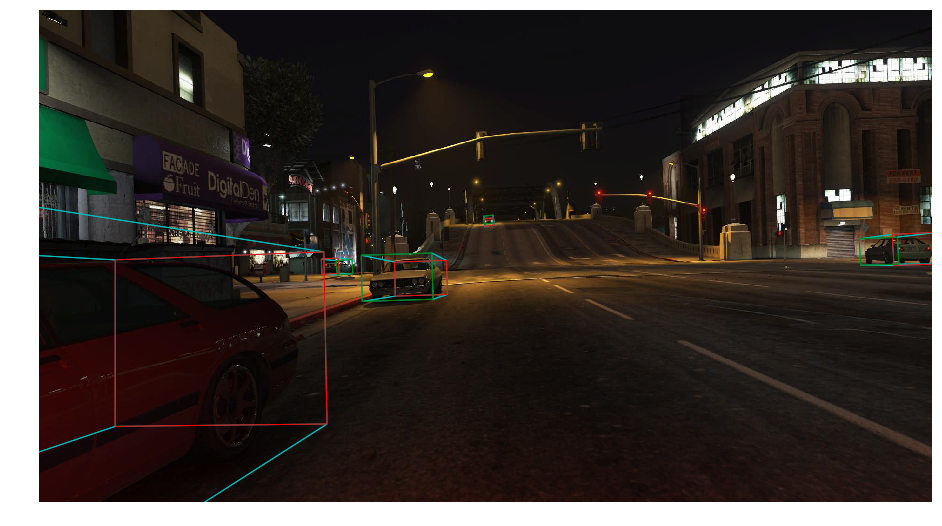
\includegraphics[scale=0.4]{obrazky/bbox-night}

\caption{3D bounding box - night}
\end{figure}
\begin{figure}
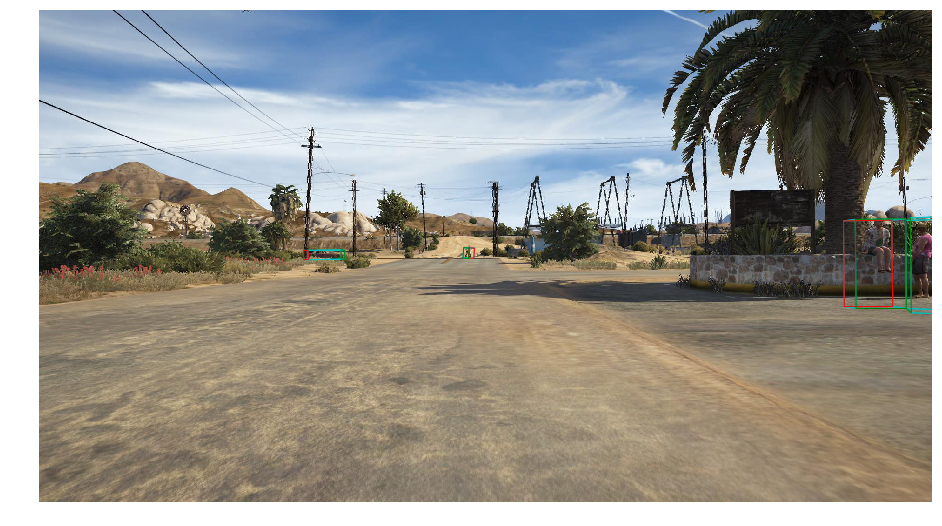
\includegraphics[scale=0.4]{obrazky/bbox-day-people}

\caption{3D bounding box - day}
\end{figure}
\begin{figure}
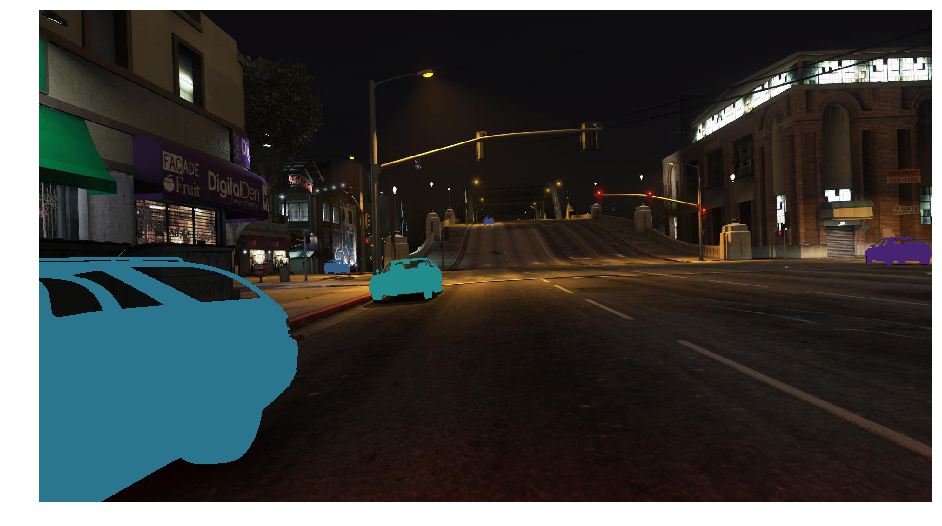
\includegraphics[scale=0.4]{obrazky/pixelwise-night}

\caption{pixel-wise annotation of cars}
\end{figure}

\begin{figure}
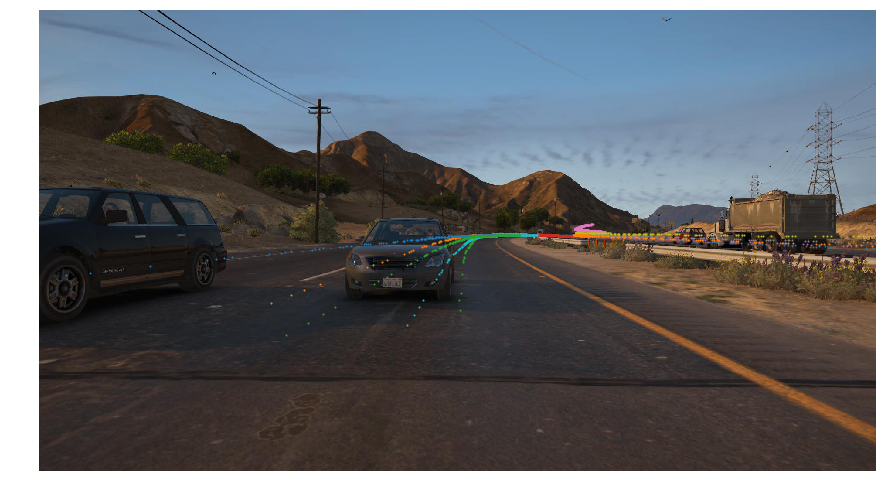
\includegraphics[scale=0.4]{obrazky/trajectories-day}

\caption{individual car trajectories}
\end{figure}


\chapter{Related work}

Richter et al. \cite{playing-for-data} used GTA V to obtain screenshots
and performed semi-automated pixel-wise semantic segmentation. Although
the process was not fully automatic, the annotation speed per image
was drastically increased, being 771 times faster than fine per-image
annotation of Cityscapes \cite{cityscapes} and 514 times faster than
per-image annotation of CamVid \cite{camvid}. Richter et al. extracted
24 966 images from game GTA V, which is roughly two orders of magnitude
larger than CamVid and three orders of magnitude larger than semantic
annotations for KITTI dataset. They trained the prediction module
of Yu and Kolthun \cite{kolthun-dilation} and by using on $\frac{1}{3}$
of the CamVid training set (which is ) and all 24 966 GTA V screenshots,
they outperformed same model trained on whole CamVid training dataset.

For images extraction, they use RenderDoc\cite{renderdoc}, stand-alone
graphics debugger. It intercepts the communication between the game
and the GPU and allows to gather screenshots. It's advantage is that
it can be used for different games, allowing to gather datasets in
various environments.

Johnson-Roberson et al. \cite{driving-in-matrix} used GTA V screenshots,
depth and stencil buffer to produce car images and automatically calculated
their bounding boxes. 

On these generated data, they trained Faster R-CNN \cite{faster-r-cnn}
only on screenshots from the GTA V game, using up to 200 000 screenshots,
which is one order of magnitude bigger than Cityscapes dataset. Using
only screenshots for training, they outperformed same architecture
trained on Cityscapes, evaluating on KITTI dataset. They developed
their own GTA V mod\ref{sec:GTA-V-modding} to hook into GPU calls
and gather screenshots from here. 

\chapter{Transforming GTA V into the State of the Art simulator}

In this thesis, Grand Theft Auto V (GTA V) game is used for creating
synthetic, nearly photo-realistic dataset. 

\section{GTA V introduction}

GTA V is action-adventure open-world video game developed by Rockstar
North and published by Rockstar Games. The game was released on 17.9.2013
for PlayStation 3 and Xbox 360\cite{gta-release} , in 18.11.2014
for PS4 and Xbox One and in 14.4.2015 it was released on PC, Windows\cite{gta-release-pc}.

The game is based on proprietary game engine, called \label{rage}RAGE
(Rockstar Advanced Game Engine)\cite{gta-5-rage}, which is used as
a base for most of Rockstar Games products. 

Till the release on Microsoft, Windows, it has been in development
for 5 years with approximate 1000-person team\cite{gta-interview-studio}.
The world of GTA V was modelled on Los Angeles\cite{gta-v-interview}
and other areas of Southern California, with road networks respecting
design of Los Angeles map. 

As could be expected from AAA game like GTA V, motion capture was
used to character's both body and facial movements. 

There are several reasons why GTA V is better for dataset creation
than other games. To use a game for dataset creation, we have multiple
requirements. The graphics of the game must be near photorealistic,
since we try to to use it instead of photos for computer vision tasks.
This disqualifies most of games, and leaves us only with AAA games
produced by big companies and few other games with State of the Art
graphics. 

The other requirement is possibility of good-enough way to interact
with the game programmatically. Usually we want to setup at least
part of the environment before gathering data. This part heavily depends
on community around the particular game.

Also the advantage of GTA V compared to some other games is abundance
of models and various sceneries in its virtual world. It has complex
transportation system of roads, highways, intersections, railroad
crossing, tunnels, and pedestrians. It also has urban, suburban, and
rural environments \cite{video-games-for-autonomous-driving}.

In gaming subculture, there are communities where people specialize
in reverse-engineering of games and development of modifications to
these games. These people are called modders or mod developers, and
these unofficial modifications and extension of games are called mods.
For few games, developers welcome this kind of activity and sometimes
they even release tools to ease the game modding. In most cases, the
game developers simply don't care and in few cases, they actively
fight against the reverse-engineering and modding. 

The GTA V is second case, where Rockstar Games does not actively try
to prevent the reverse-engineering, but they don't release any tools
to ease it, either. This results in cyclic process of Rockstar Games
releasing new version of game, including backward compatibility (BC)
breaks, and community reverse engineering the new version and adjusting
their mods to work with the new version.

The modding community around the GTA V is based mostly on community
around GTA IV, which was previous big game produced by Rockstar Games.
So many tools are just GTA IV based and only modified to work with
GTA V. Luckily, the community is large and productive, so we have
many mods and many function in GTA V reverse-engineered and thus prepared
for programmatic interactions.

\subsection{Cars}

There is big variety of cars models. Specifically, the are 259 car
models, all of them are listed here \cite{gta-vehicle-models}. These
models cars of various shapes and sizes, from golf carts to trucks
and trailers. This diversity is representative of real distribution
of vehicles. It even allows us to simulate environments with various
types of vehicles, which would be very difficult in real environment.
GTA V provides us many information about cars, more on this will be
covered in section \ref{sec:GTA-V-data-obtaining}.

\subsection{Pedestrians}

GTA V has pedestrians and provides some information about them, more
on this in section \ref{sec:GTA-V-data-obtaining}. The game has pedestrians
of both genders and various ethnicities. Pedestrians appear in various
poses, like standing, walking, sitting, many animations etc. The main
drawback of GTA V is that all pedestrians are about the same height\cite{video-games-for-autonomous-driving}.

\section{Automotive Simulators}

Currently, there are some open-source simulation platforms for automotive
industry which could be theoretically used for creating synthetic
datasets. But compared to AAA games like GTA V, they have much less
resources and much less customers to finance the development. In result,
simulators have worse graphics than AAA games and NPC (non playable
characters) don't have as sophisticated behaviour. In GTA V, drivers
mostly follow traffic regulations, traffic lights and traffic lanes,
which leafs to very realistic environment better than simulators can
provide.

\section{\label{sec:GTA-V-modding}GTA V modding ecosystem}

Although the modding community is quite big, as it is in lots of open-source
communities, essential part of community depends on one person. Here,
it is Alexander Blade. In his free time, he reverse-engineered big
part of GTA V and developed ScriptHookV\cite{scripthookv-gtaforums},
library enabling to perform native calls into GTA V in C++ and develop
GTA V mods in C++. Currently, more people in community participates
in reverse-engineering and they share their knowledge in GTA forum
thread\cite{nativedb-research}.

List of all reverse-engineered native functions is kept in following
list \cite{nativedb}. Assumably, GTA V contains \textasciitilde{}5200
natives. There is no original native name list of functions in GTA
V, name hashes are used instead. During reverse-engineering and game
decompilation, \textasciitilde{}2600 native names were discovered
using brute-force and manual checking afterwards. For these functions,
number of parameters and returns of these calls are also known. In
the native functions list, for big part of functions we know their
name, signature and how do they affect the game. The rest remains
to be discovered yet.

When new version of game is released, in few days to weeks, new version
of ScriptHookV is released, fixing BC breaks.

Other heavily used mod in community is ScriptHookDotNet2, which is
built atop of ScriptHookV and creates bridge between C\# language
and ScriptHookV, effectively allowing to write GTA V mods in C\#.
It is available as open-source \cite{scripthookvdotnet}. Along with
creating bridge between C\# and GTA V, it wraps most used native calls
into classes, leveraging object-oriented paradigm for mod development
using getters and setters as proxies for native calls. 

Next notable mod is NativeUI\cite{nativeui}. It renders windows atop
of GTA V GUI and allows us to define custom control panels for manipulating
custom functionality in other mods. 

Unlike most of other mods, these three mods act more as a framework
for mod development. 

Since GTA V is a game, it requires human interaction. For simulator-like
behaviour we would want the car to drive autonomously to crawl data
without human interaction. This can be done using VAutodrive\cite{vautodrive}.
This allows us to use NPC automatic behaviour patterns for main player,
letting the player randomly wander the world, even in car, without
need of human assistance during crawling. Unfortunately, this package
is not open-source.

Generally, the community is not united in their view on open-source.
Some mods are available open-source on GitHub. Other mods are being
distributed only as compiled binaries\cite{gta-5-mods}. Lots of modders
develop mostly by trial and error, and no comprehensive documentation
for mod development is available, unfortunately. There are some tutorials
\cite{gta-5-mod-tutorial}, but they are far from complete and provide
only basic knowledge, leaving reader without deeper understanding
of underlying principles.

Modders mostly meet online on few GTA forums, where they exchange
knowledge \cite{gta-forums,gta-5-mods-forum}. GitHub or Stack Overflow,
which are biggest information sources for usual software development,
are not used much in GTA modding community. Due to this fact, these
forums, along with source code of open-source mods comprise knowledge-base
of mod development.

\section{Simulation environment and development stack}

In this thesis, I use mod based on \cite{driving-in-matrix} but enhanced
to gain more control of the game and to obtain more information from
the game. 

In later text, I'll refer to some GTA V native functions or data structures
which are output of GTA V native functions. To be consistent and to
help understanding, I will use function names from native function
list \cite{nativedb}.

The basic architecture of C\# mods come from the ScriptHookDotNet2,
where each mod script extends the GTA.Script class. For each child
of this class, we can set integer Interval, Tick and KeyUp callbacks.
Interval property determines how big interval in milliseconds is between
consecutive Tick calls. Tick callback is being called periodically,
so here we can set tasks which we want to perform periodically, e.g.
screenshot gathering. The KeyUp callback is for interacting with user
and reading the user's keyboard input. For data gathering mods, this
is mostly used for debugging purposes, script disabling or restarting. 

Little, but useful note for debugging and developing scripts based
on ScriptHookDotNet2: when changing mod compiled binaries, we don't
have to restart the game for newer version of mod to be active. Pressing
Insert causes all C\# binaries to reload, causing new version of source
code to load into game, which dramatically decreases time of feedback
loop during development. This does not work for C++ mods and compiled
.asi files.

todo: popsat sem architekturu

\section{\label{sec:GTA-V-data-obtaining}GTA V native API and data obtaining}

The data obtained from GTA V can be divided into multiple categories.
\begin{itemize}
\item Image data
\item Rendering pipeline matrices
\item GTA V internal data
\begin{itemize}
\item entities
\item camera
\item player
\item other data via API
\end{itemize}
\end{itemize}

\subsection{Image data}

There are 3 image data. RGB image, depth image and stencil image.

RGB image is usual camera image. Depth image is content of GPU's depth
buffer, in NDC. More detailed description of depth values is in subsection
\ref{subsec:Camera-to-NDC}. The last is pixel-wise stencil buffer.
The stencil semantics is explained in the next paragraph.

\subsubsection{Stencil data}

Stencil buffer contains auxiliary data per pixel. It is 8bit unsigned
integer, where 1.-4. bits (counting from LSB) contain object type
ID, and 5.-8. bits contain certain flags. 

That means there are 15 object types and 4 flags. 

For some object type IDs, I reverse engineered its semantics based
on corresponding RGB image. 
\begin{center}
\begin{tabular}{|c|c|c|}
\hline 
Object type ID binary & Object type ID decimal & Semantics\tabularnewline
\hline 
\hline 
0000 & 0 & background (buildings, roads, hills...)\tabularnewline
\hline 
0001 & 1 & pedestrian\tabularnewline
\hline 
0010 & 2 & vehicle\tabularnewline
\hline 
0011 & 3 & tree, grass\tabularnewline
\hline 
0111 & 7 & sky\tabularnewline
\hline 
\end{tabular}
\par\end{center}

The background, pedestrian and vehicle IDs are most important for
vehicles detection and semantic segmentation, and other object types
are not so valuable for these tasks, which is why I didn't investigate
further in semantics and they remain to be reverse-engineered.

For stencil flags, semantics was discovered for half of them. 
\begin{center}
\begin{tabular}{|c|c|c|}
\hline 
position of bit & position in whole stencil value & Semantics\tabularnewline
\hline 
\hline 
5 & xxx1xxxx & artificial light source\tabularnewline
\hline 
8 & 1xxxxxxx & player's character\tabularnewline
\hline 
\end{tabular}
\par\end{center}

Sample stencil image can be seen in \ref{fig:Visualization-pipeline}.
\begin{center}
\begin{figure}
\begin{centering}
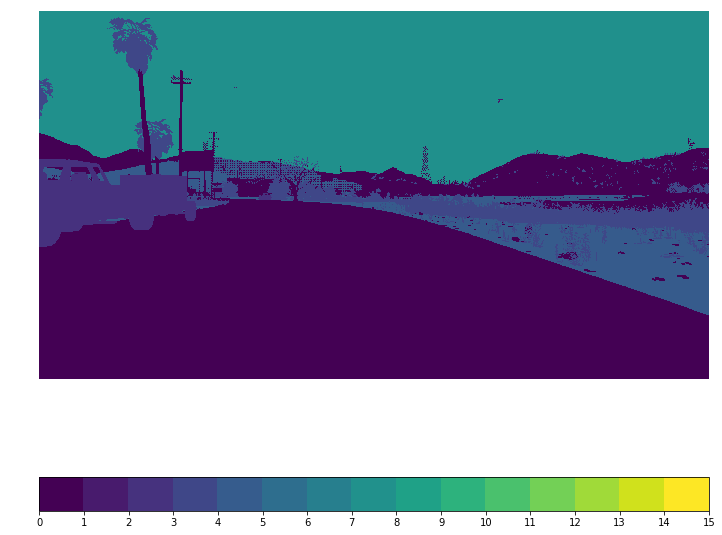
\includegraphics[width=12cm]{obrazky/2018-03-30--06-00-56--114-stencil-color-ids}
\par\end{centering}
\begin{centering}
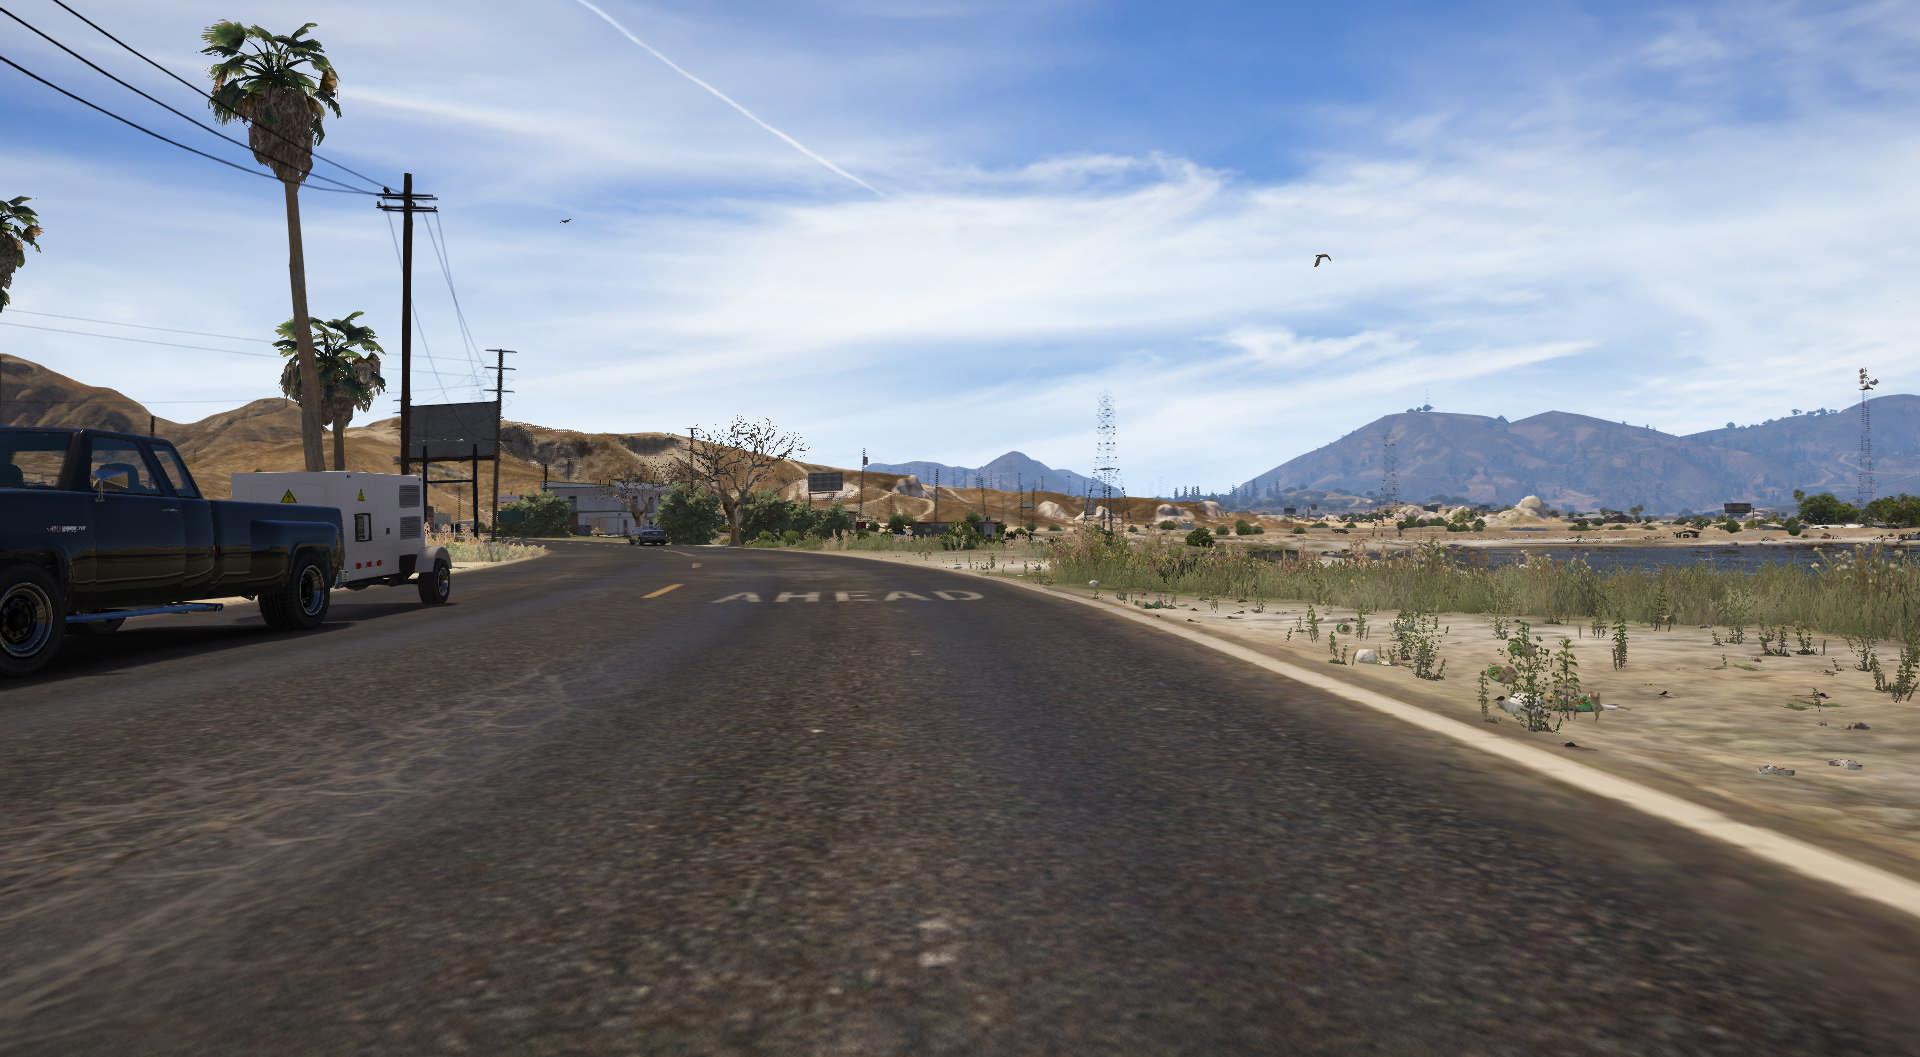
\includegraphics[width=12cm]{obrazky/2018-03-30--06-00-56--114}
\par\end{centering}
\caption{\label{fig:Sample-stencil-object}Sample stencil object types image
and corresponding RGB image}
\end{figure}
\par\end{center}

\subsubsection{Extracting images from GPU's internal buffers}

To understand how the image gathering works, we need to dive deeper
into Microsoft Windows graphics.

In Microsoft Windows, the main graphics engine is DirectX (roughly
Windows equivalent of OpenGL). One part of DirectX is Direct3D, which
is used to render 3D graphics with hardware acceleration, and most
importantly, it provides graphics API. The whole process of obtaining
image data is done by mod provided as part of the paper \cite{driving-in-matrix}.
The mod has two parts, called native and managed plugin.

Image data is being obtained by native plugin by hooking into Direct3D
11's present callback. That means the native call is replaced with
custom code, which is being executed and then returns to the native
call. In that custom code, content of GPU's buffers is copied. Specifically,
the depth and stencil data are captured by hooking into Direct3D’s
ID3D11ImmediateContext:: ClearDepthStencilView and saving the buffers
before each call. Because of optimizations applied by the graphics
card drivers, the function needs to be re-hooked into the clear function
each frame. When saving each sample, the managed plugin requests all
current buffers from the native plugin and the buffers are downloaded
from the GPU and copied into managed memory.\cite{driving-in-matrix}. 

\subsection{\label{subsec:Rendering-pipeline-data}Rendering pipeline data}

Direct3D allows us to get rendering pipelines through the D3D11\_MAP\_READ
call. This way, the world, world-view, and world-view-projection matrices
are obtained. Let's denote them as world matrix = $W$, world-view
by = $VW$, and world-view-projection = $PVW$. We need to get individual
matrices, which we obtain by multiplication by matrices inversion:
\begin{align*}
V & =VW\cdot W^{-1}\\
P & =PVW\cdot\left(VW\right)^{-1}=PV\cdot W^{-1}\cdot V^{-1}
\end{align*}

View and projection matrices are important on their own, without the
world matrix. Their semantics and importance is more described in
section \ref{sec:Reverse-engineering-the-RAGE}. These matrices can
be simply obtained by inversion as stated above. But this approach
is not numerically stable, and sometimes causes resulting matrix to
be incorrect and not usable for further usage. Another caveat of this
approach is that during data gathering in higher speeds, the native
call becomes laggy and resulting matrices are highly imprecise. Although
we can obtain these matrices via the native call, they can be reconstructed
with higher precision, as described in \ref{sec:Reverse-engineering-the-RAGE}.

\subsection{GTA V internal data}

These data are probably most valuable compared to data gathering by
other methods. In this section, I describe which data about various
game objects can be obtained and how to obtain them. 

All data in this section are obtained though native calls into GTA
V, which are listed here \cite{nativedb}. As mentioned above, they
can be called from C++ and C\#. For convenience, and because most
of my mod development is done in C\#, I will also describe the C\#
wrappers. The ScriptHookDotNet2\cite{scripthookvdotnet} wrapper heavily
uses object properties. The C\# API is divided into multiple classes,
listed \href{https://github.com/crosire/scripthookvdotnet/tree/dev_v3/source/scripting}{here}.
Each class has properties, whose getters and setters are implemented
as calling the native functions. This feature is nice tooling and
leads to more readable and maintainable code. I will describe parts
of API which are most useful for synthetic datasets creation.

\subsubsection{Coordinate systems and axes}

The model, world and view coordinate systems are all in meters. In
the model coordinate system, e.g. when we have coordinate system of
a car, Z-axis is oriented upwards, Y-axis is oriented in front of
the car, and X-axis to the right of the car. In the camera coordinate
system, the Z-axis is oriented behind the camera, Y-axis upwards of
camera and the X-axis to the left of camera. In the world coordinate
system, if the camera has rotation = $\left(0,0,0\right)$, it is
heading in direction of Y-axis, X-axis is heading right of the camera,
and Z axis is heading upwards.

\subsubsection{Game state manipulation}

In the ScriptHookVDotNet2, where is Game class, which is the main
entry-point for most of game state manipulation. Here I'll describe
methods and properties useful and needed for data retrieval.
\begin{lyxcode}
Game.Pause(true)
\end{lyxcode}
pauses the whole game. 
\begin{lyxcode}
Game.Pause(false)
\end{lyxcode}
un-pauses the game. The 

\code{Game.ScreenResolution}

property returns Size object with height and width of the current
screen, so 
\begin{lyxcode}
Game.ScreenResolution.Width;~Game.ScreenResolution.Height;
\end{lyxcode}
returns screen width and height respectively. As seen above, the main
player character can be accessed by \code{Game.Player.Character}
property. 

The Player Character property is used for handling the main player.
It has following method important for data retrieval. \code{Game.Player.Character.Position}
provides position of player in world coordinates. This is useful if
we want to obtain entities only in certain distance of player or if
we want to spawn new vehicle on player's position. Similarly to position,
we can access player's current velocity by 
\begin{lyxcode}
Game.Player.Character.Velocity
\end{lyxcode}
which returns the velocity 3D vector. If we have a vehicle, we set
the player as driver as follows 
\begin{lyxcode}
Game.Player.Character.SetIntoVehicle(vehicle,~

VehicleSeat.Driver)
\end{lyxcode}
. When player is in a vehicle, we can access it later by the 
\begin{lyxcode}
Game.Player.Character.CurrentVehicle
\end{lyxcode}
property. 

Other important Class is World, which, as seen above, provides the
camera handling interface, and many other features. As mentioned above,
the World.DestroyAllCameras() clears all scripted cameras. The \code{World.CreateCamera()}
creates new scripted camera. The \code{World.RenderingCamera} holds
reference to the currently active scripted camera. Setting the camera
to the \code{World.RenderingCamera} activates that camera and starts
rendering with that camera, and setting null reference returns the
view to the Gameplay camera, which is default camera used during playing. 

Other methods allow us directly manipulate the world. The \code{World.CurrentDayTime}
returns the TimeSpan object, which is time in day in the GTA world.
By setting this property we can change the time of day as we need
by assigning the TimeSpan instance 
\begin{lyxcode}
World.CurrentDayTime~=~

new~TimeSpan(int~hours,~int~minutes,~int~seconds)
\end{lyxcode}
. The \code{World.Weather} uses same getter, setter interface, so
\code{World.Weather} returns current weather, and \code{World.Weather = Weather.Foggy}
sets the weather to be foggy. List of all possible weathers is in
the Weather enum, which contains Unknown, ExtraSunny, Clear, Clouds,
Smog, Foggy, Overcast, Raining, ThunderStorm, Clearing, Neutral, Snowing,
Blizzard, Snowlight, Christmas, Halloween. 

The World class also contains the 
\begin{lyxcode}
World.CreateVehicle(Model~model,~Vector3~position)
\end{lyxcode}
which spawn new car in the game and returns reference to the newly
spawned car. Position is in world coordinates and model can be any
of vehicle models in game. For instance,
\begin{lyxcode}
World.CreateVehicle(new~Model(VehicleHash.Seven70),~

Game.Player.Character.Position)
\end{lyxcode}
creates new sports car in player's position . Whole list of known
models is available in \url{https://github.com/crosire/scripthookvdotnet/blob/dev_v3/source/scripting/World/Entities/Vehicles/VehicleHash.cs}
where 554 model hashes are enumerated. 

\subsubsection{Camera}

The camera is probably one of the most crucial parts of the API. There
is Gameplay Camera, which is the default camera used during usual
playing. This camera can be manipulated, but its usage is limited.
Other approach is usage of scripted cameras, which can be fully controlled
programmatically. We can create multiple scripted cameras and switch
between them, but the community discovered there is hard limit of
26 cameras at time\cite{gta-mod-camera}. Camera can be created by
calling 
\begin{lyxcode}
Camera~camera~=~World.CreateCamera(

new~Vector3(x,~y,~z),~new~Vector3(x,~y,~z),~float~fov);
\end{lyxcode}
which returns handle to the new camera. The position is in world coordinates
in meters. The rotation is in degrees as rotation around particular
axis, as in OpenGL engine. In the Aircraft principal axes terminology,
the $\left(x,y,z\right)$ rotation vector means $\left(pitch,roll,yaw\right)$
respectively. The fov argument is vertical field of view in degrees.
The default value is 50. One can of course call the underlying native
functions directly, but this wrapper helps with managing the handles. 

All scripted cameras can be destroyed by calling the 
\begin{lyxcode}
World.DestroyAllCameras();~
\end{lyxcode}
Switching to the scripted camera can be done by calling 
\begin{lyxcode}
camera.IsActive~=~true;
\end{lyxcode}
, and switching from this camera to some other by 
\begin{lyxcode}
camera.IsActive~=~false;~
\end{lyxcode}
Right after creating the camera, when we don't to switch to this camera
immediately, we need to deactivate it by these two lines of code
\begin{lyxcode}
camera.IsActive~=~false;

World.RenderingCamera~=~null;
\end{lyxcode}
this code ensures that camera is created properly. We don't know precisely,
why is this needed, but this is the price for using the closed and
reverse-engineered codebase. By calling the
\begin{lyxcode}
camera.IsActive~=~true;~

World.RenderingCamera~=~camera;
\end{lyxcode}
scripted camera becomes active and view is switched to this camera.
All properties of camera can be set simply by calling setters
\begin{lyxcode}
camera.position~=~new~Vector3(x,~y,~z);

camera.rotation~=~new~Vector3(y,~x,~z);

camera.nearClip~=~distance;

camera.farClip~=~distance;

camera.FieldOfView~=~fov;
\end{lyxcode}
and read by calling getters 
\begin{lyxcode}
Vector3~position~=~camera.position;

Vector3~rotation~=~camera.rotation;

float~distance~=~camera.nearClip;

float~distance~=~camera.farClip;

float~fov~=~camera.FieldOfView;
\end{lyxcode}
The near clip and far clip is again in meters. So we can set all needed
parameters simply by calling getters and setters. So if we want to
use camera, we simply set parameters and then activate it. This creates
the static camera. 

Sometimes we want the camera to be moving, e.g. when gathering data
by driving car. Camera can be attached to any entity by calling 
\begin{lyxcode}
camera.AttachTo(entity,~new~Vector3(x,~y,~z));
\end{lyxcode}
the second parameter is relative offset to middle of the attached
entity. The offset is in model coordinate system which means its position
moves and rotates with attached entity. During dataset gathering,
I used this code
\begin{lyxcode}
camera.AttachTo(Game.Player.Character.CurrentVehicle,~

new~Vector3(0f,~2f,~0.4f));
\end{lyxcode}
to attach camera to the front part of player's current vehicle. As
seen from code, it attaches camera 2 meters in front of mar model's
centre and 40cm above it, making it effectively sitting on top of
the hood of the car. These parameters are taken from \cite{video-games-for-autonomous-driving}. 

When we have camera attached to the car, we need to update periodically
its rotation, otherwise it will be heading the same direction in world
coordinates and won't rotate with car it is attached to. So when we
have our Tick method, which is being called periodically, we need
to update the active camera like this:
\begin{lyxcode}
camera.AttachTo(Game.Player.Character.CurrentVehicle,~

cameraPosition);

camera.Rotation~=~cameraRotation;
\end{lyxcode}
if we want to have our camera rotated in fixed offset compared to
car rotation (e.g. camera looking behind the car), we simply set camera's
rotation as offset like this
\begin{lyxcode}
camera.AttachTo(Game.Player.Character.CurrentVehicle,~

new~Vector3(0f,~-2f,~0.6f));~~//~now~our~camera~is~sitting~in~back~of~the~car

camera.Rotation~=~Game.Player.Character.CurrentVehicle.Rotation~

+~new~Vector3(0f,~0f,~180f);
\end{lyxcode}
which sets camera rotation in world coordinates as a sum of car's
rotation and relative rotation of camera, 180\textdegree{} yaw.

\subsubsection{Game entities}

All game entities extend the abstract Entity class. Important children
of Entity class are Ped, Vehicle and Prop classes, wrapping pedestrians,
vehicles, and various objects, respectively. List of all entities
contained in the entity pool can be obtained by \code{World.GetAllEntities()}.
Methods 
\begin{lyxcode}
World.GetAllPeds();~World.GetAllVehicles();~World.GetAllProps();
\end{lyxcode}
will return list of all pedestrians, vehicles, and props, respectively.
These lists are huge and we don't need all of returned entities usually.
Most of the time, we are interested only in objects on the screen,
which are only in certain distance from us. The most straightforward
option is to filter these lists afterwards, but luckily, the library
offers us helper methods for filtering the nearby entities more effectively,
without need to instantiate more distant entities. These helper methods
are 
\begin{lyxcode}
World.GetNearbyEntities(Vector3~position,~float~radius)
\end{lyxcode}
, and analogously, 
\begin{lyxcode}
World.GetNearbyPeds(Vector3~position,~float~radius);~

World.GetNearbyVehicles(Vector3~position,~float~radius);~

World.GetNearbyProps(Vector3~position,~float~radius);
\end{lyxcode}
. As expected, radius is in meters, position is in world coordinates.
So obtaining for instance all vehicles up to half kilometres distant
from the current player, we call 
\begin{lyxcode}
World.GetNearbyVehicles(Game.Player.Character,~500.0f)
\end{lyxcode}
. Every entity has position, rotation, velocity, and handle. Position
and rotation have similar semantics as cameras. Velocity is velocity
as a 3D vector. The handle is unique in-game identifier of particular
entity, allowing identifying it across whole game during data gathering,
and lets us identify same entity on multiple images, which is useful
for identifying motion of entity through different images. By calling
\code{entity.Model.Hash} on a particular entity, we obtain its hash,
which can be used to spawn new entities with same model. For vehicles,
there is \code{entity.ClassType} property, describing type as one
of 21 vehicle types. Whole list can be seen in the enum VehicleClass
in the \url{https://github.com/crosire/scripthookvdotnet/blob/dev_v3/source/scripting/World/Entities/Vehicles/Vehicle.cs}. 

\subsubsection{Gathering data from active camera}

In this part, I'll describe how to access data from internal GPU buffers
and how to persist these data. 

Before we gather buffers contents, we want to pause the game. Since
we don't get the data from buffers perfectly synchronized, we pause
the game to make sure RGB, depth and stencil buffer contain data coming
from same frame. \code{Game.Pause(true)} pauses the game. The whole
data retrieval from buffers is done via GTAVisionExport native plugin
\cite{driving-in-matrix}. When the game is stopped, we can obtain
RGB, depth and stencil buffer contents by 
\begin{lyxcode}
var~color~=~VisionNative.GetColorBuffer();

var~depth~=~VisionNative.GetDepthBuffer();

var~stencil~=~VisionNative.GetStencilBuffer();~
\end{lyxcode}
and then, we save it to the filesystem as TIFF image. Although TIFF
is not the most used format for data, it is able to persist image
whose pixels contain float values, which is crucial for depth buffer.

The RGB buffer is usual 8bit unsigned integer RGBA image. The depth
buffer contains float values, with 32bits precision, in range from
0 to 1, representing depth value in NDC space. The stencil buffer
contains 8bit unsigned integer image. 

\section{\label{sec:Reverse-engineering-the-RAGE}Reverse-engineering the
RAGE rendering pipeline}

As mentioned above \ref{rage}, GTA V uses proprietary game engine,
Rockstar Advanced Game Engine (RAGE). The basic premise of rendering
pipeline is same as in well known graphics engines like OpenGL. The
pipeline is shown in figure \ref{fig:Visualization-pipeline}. Following
section will be discussing mostly computer graphics related problems.
Due to some terminology inconsistency between computer graphics and
computer vision, all terms used here will be computer graphics related.
Probably most confusion here could be caused by projection matrix.
In computer vision, projection matrix is projection from 3D to 2D,
the matrix reduces dimension. In computer graphics, all coordinates
are kept in 4D, in homogeneous coordinates as long as possible. Here
the projection matrix represents projection from frustum seen by eye
into cuboid space of Normalized Device Coordinates.

\begin{figure}
\begin{centering}
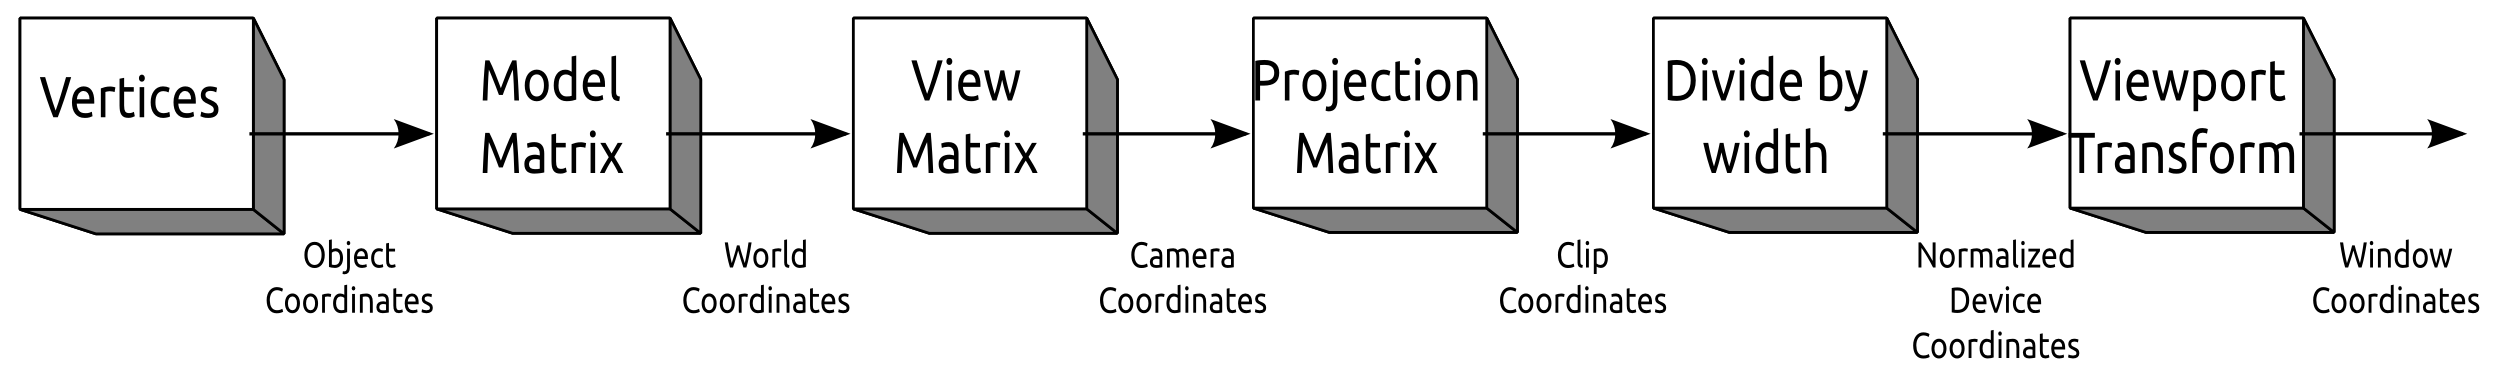
\includegraphics[scale=0.65]{obrazky/transformationPipeline}
\par\end{centering}
\caption{\label{fig:Visualization-pipeline}Rendering pipeline}
\end{figure}
In is part, I will describe some transformations between individual
RAGE coordinate systems. Some points here will have part of name in
lower index. The name of coordinate system will be denoted in upper
index. In RAGE there are 6 coordinate systems.
\begin{center}
\begin{tabular}{|c|c|c|}
\hline 
Name & Abbreviation & Example point $x$\tabularnewline
\hline 
\hline 
Object Coordinates & O & $x^{O}$\tabularnewline
\hline 
World Coordinates & W & $x^{W}$\tabularnewline
\hline 
Camera Coordinates & C & $x^{C}$\tabularnewline
\hline 
Clip Coordinates & L & $x^{L}$\tabularnewline
\hline 
Normalized Device Coordinates & NDC & $x^{NDC}$\tabularnewline
\hline 
Windows Coordinates & P & $x^{P}$\tabularnewline
\hline 
\end{tabular}
\par\end{center}

Most of points we handle in GTA already are in world coordinates. 

But some points, like GAMEPLAY::GET\_MODEL\_DIMENSIONS

$=\begin{pmatrix}x_{max}^{O} & y_{max}^{O} & z_{max}^{O}\end{pmatrix}\begin{pmatrix}x_{min}^{O} & y_{min}^{O} & z_{min}^{O}\end{pmatrix}$
output, are in object coordinates. Transitions between adjacent coordinate
systems will be demonstrated on model dimensions because it is on
the few vectors which are obtained in Object Coordinates and there
is need to project them into Window Coordinates.

\subsection{Object to World Coordinates}

To get world coordinates of model dimensions, we use traditional rigid
body transformation based on ENTITY::GET\_ENTITY\_ROTATION$=\begin{pmatrix}\alpha & \beta & \gamma\end{pmatrix}$
Euler angles, 

and ENTITY::GET\_ENTITY\_COORDS$=\begin{pmatrix}x^{W} & y^{W} & z^{W}\end{pmatrix}$.

Because all coordinates will be homogeneous coordinates, the above-mentioned
model dimensions vectors will be transformed to following form $\begin{pmatrix}x_{max}^{O} & y_{max}^{O} & z_{max}^{O} & 1\end{pmatrix}\begin{pmatrix}x_{min}^{O} & y_{min}^{O} & z_{min}^{O} & 1\end{pmatrix}$. 

The transition is represented by model matrix
\begin{align*}
M & =\begin{bmatrix}1 & 0 & 0 & x^{W}\\
0 & 1 & 0 & y^{W}\\
0 & 0 & 1 & z^{W}\\
0 & 0 & 0 & 1
\end{bmatrix}\begin{bmatrix}1 & 0 & 0 & 0\\
0 & \cos\left(\alpha\right) & -\sin\left(\alpha\right) & 0\\
0 & \sin\left(\alpha\right) & \cos\left(\alpha\right) & 0\\
0 & 0 & 0 & 1
\end{bmatrix}\begin{bmatrix}\cos\left(\beta\right) & 0 & \sin\left(\beta\right) & 0\\
0 & 1 & 0 & 0\\
-\sin\left(\beta\right) & 0 & \cos\left(\beta\right) & 0\\
0 & 0 & 0 & 1
\end{bmatrix}\begin{bmatrix}\cos\left(\gamma\right) & -\sin\left(\gamma\right) & 0 & 0\\
\sin\left(\gamma\right) & \cos\left(\gamma\right) & 0 & 0\\
0 & 0 & 1 & 0\\
0 & 0 & 0 & 1
\end{bmatrix}\\
 & =\begin{bmatrix}\cos\left(\beta\right)\cos\left(\gamma\right) & -\cos\left(\beta\right)\sin\left(\gamma\right) & \sin\left(\beta\right) & x^{W}\\
\sin\left(\alpha\right)\sin\left(\beta\right)\cos\left(\gamma\right)+\cos\left(\alpha\right)\sin\left(\gamma\right) & \cos\left(\alpha\right)\cos\left(\gamma\right)-\sin\left(\alpha\right)\sin\left(\beta\right)\sin\left(\gamma\right) & -\sin\left(\alpha\right)\cos\left(\beta\right) & y^{W}\\
\sin\left(\alpha\right)\sin\left(\gamma\right)-\cos\left(\alpha\right)\sin\left(\beta\right)\cos\left(\gamma\right) & \cos\left(\alpha\right)\sin\left(\beta\right)\sin\left(\gamma\right)+\sin\left(\alpha\right)\cos\left(\gamma\right) & \cos\left(\alpha\right)\cos\left(\beta\right) & z^{W}\\
0 & 0 & 0 & 1
\end{bmatrix}
\end{align*}

and whole transformation is, as expected 
\[
M\begin{bmatrix}x_{max}^{O} & x_{min}^{O}\\
y_{max}^{O} & y_{min}^{O}\\
z_{max}^{O} & z_{min}^{O}\\
1 & 1
\end{bmatrix}=\begin{bmatrix}x_{max}^{W} & x_{min}^{W}\\
y_{max}^{W} & y_{min}^{W}\\
z_{max}^{W} & z_{min}^{W}\\
w_{max}^{W} & w_{min}^{W}
\end{bmatrix}
\]


\subsection{World to Camera Coordinates}

The transformation from world coordinates is principally the same,
but counter-intuitive in definition of used rotation matrices. It
also is rigid body transformation, but rotation is defined differently
than we are usually used to in computer graphics. The rotation matrices
were reverse engineered as part of this thesis from camera position,
rotation and resulting view matrix, this coordinate system is nowhere
else documented. The camera position is CAM::GET\_CAM\_COORD$=\begin{pmatrix}x^{W} & y^{W} & z^{W}\end{pmatrix}$
and the camera rotation is CAM::GET\_CAM\_ROT$=\begin{pmatrix}\alpha & \beta & \gamma\end{pmatrix}$.

The transformation is represented by view matrix
\begin{align*}
V & =\begin{bmatrix}1 & 0 & 0 & 0\\
0 & \sin\left(\alpha\right) & \cos\left(\alpha\right) & 0\\
0 & \cos\left(\alpha\right) & -\sin\left(\alpha\right) & 0\\
0 & 0 & 0 & 1
\end{bmatrix}\begin{bmatrix}\cos\left(\beta\right) & 0 & -\sin\left(\beta\right) & 0\\
0 & 1 & 0 & 0\\
\sin\left(\beta\right) & 0 & \cos\left(\beta\right) & 0\\
0 & 0 & 0 & 1
\end{bmatrix}\begin{bmatrix}\cos\left(\gamma\right) & \sin\left(\gamma\right) & 0 & 0\\
\sin\left(\gamma\right) & -\cos\left(\gamma\right) & 0 & 0\\
0 & 0 & 1 & 0\\
0 & 0 & 0 & 1
\end{bmatrix}\begin{bmatrix}1 & 0 & 0 & x^{W}\\
0 & 1 & 0 & y^{W}\\
0 & 0 & 1 & z^{W}\\
0 & 0 & 0 & 1
\end{bmatrix}
\end{align*}
to fit the matrix into page, let us propose following substitutions 

\[
\cos\left(\alpha\right)=c_{\alpha},sin\left(\alpha\right)=s_{\alpha}
\]

\[
\cos\left(\beta\right)=c_{\beta},sin\left(\beta\right)=s_{\beta}
\]

\[
\cos\left(\gamma\right)=c_{\gamma},sin\left(\gamma\right)=s_{\gamma}
\]
\begin{align*}
V & =\begin{bmatrix}c_{\beta}c_{\gamma} & c_{\beta}s_{\gamma} & -s_{\beta} & 0\\
c_{\alpha}s_{\beta}c_{\gamma}+s_{\alpha}s_{\gamma} & c_{\alpha}s_{\beta}s_{\gamma}-s_{\alpha}c_{\gamma} & c_{\alpha}c_{\beta} & 0\\
c_{\alpha}s_{\gamma}-s_{\alpha}s_{\beta}c_{\gamma} & -s_{\alpha}s_{\beta}s_{\gamma}-c_{\alpha}c_{\gamma} & -s_{\alpha}c_{\beta} & 0\\
0 & 0 & 0 & 1
\end{bmatrix}\begin{bmatrix}1 & 0 & 0 & x^{W}\\
0 & 1 & 0 & y^{W}\\
0 & 0 & 1 & z^{W}\\
0 & 0 & 0 & 1
\end{bmatrix}\\
 & =\begin{bmatrix}c_{\beta}c_{\gamma} & c_{\beta}s_{\gamma} & -s_{\beta} & x^{W}c_{\beta}c_{\gamma}+y^{W}c_{\beta}s_{\gamma}-z^{W}s_{\beta}\\
c_{\alpha}s_{\beta}c_{\gamma}+s_{\alpha}s_{\gamma} & c_{\alpha}s_{\beta}s_{\gamma}-s_{\alpha}c_{\gamma} & c_{\alpha}c_{\beta} & x^{W}\left(c_{\alpha}s_{\beta}c_{\gamma}+s_{\alpha}s_{\gamma}\right)+y^{W}\left(c_{\alpha}s_{\beta}s_{\gamma}-s_{\alpha}c_{\gamma}\right)+z^{W}c_{\alpha}c_{\beta}\\
c_{\alpha}s_{\gamma}-s_{\alpha}s_{\beta}c_{\gamma} & -s_{\alpha}s_{\beta}s_{\gamma}-c_{\alpha}c_{\gamma} & -s_{\alpha}c_{\beta} & x^{W}\left(c_{\alpha}s_{\gamma}-s_{\alpha}s_{\beta}c_{\gamma}\right)+y^{W}\left(-s_{\alpha}s_{\beta}s_{\gamma}-c_{\alpha}c_{\gamma}\right)-z^{W}s_{\alpha}c_{\beta}\\
0 & 0 & 0 & 1
\end{bmatrix}
\end{align*}

and whole transformation is, as expected 
\[
V\begin{bmatrix}x_{max}^{W} & x_{min}^{W}\\
y_{max}^{W} & y_{min}^{W}\\
z_{max}^{W} & z_{min}^{W}\\
w_{max}^{W} & w_{min}^{W}
\end{bmatrix}=\begin{bmatrix}x_{max}^{C} & x_{min}^{C}\\
y_{max}^{C} & y_{min}^{C}\\
z_{max}^{C} & z_{min}^{C}\\
w_{max}^{C} & w_{min}^{C}
\end{bmatrix}
\]

From definition of rotation axes in the rotation matrices, following
observation can be made. $z^{C}$ represents distance from camera
in direction of camera heading, and $x^{C}$and $y^{C}$ represent
horizontal and vertical position of point relative to camera, respectively.
But the view frustum of camera is in opposite direction than $z^{C}$axis,
which means the camera ``is looking'' into negative $z^{C}$ coordinates.

\subsection{\label{subsec:Camera-to-NDC}Camera to NDC}

This is the first transformation which is not rigid-body transformation.
Because camera sees only frustum, this transformation represents transition
from frustum to cuboid in Normalized Device Coordinates. The frustum
being projected is specified by near clip, far clip, field of view
and screen resolution width and height. Usually, none of these parameters
are changing during the game, so the projection matrix is usually
the same for multiple scenes during data gathering session. Although
all of these parameters can be changed programmatically if needed. 

The near clip and far clip of camera can be obtained by \label{native-call-near-clip}
CAM::GET\_CAM\_NEAR\_CLIP$=n_{c}$ and CAM::GET\_CAM\_FAR\_CLIP$=f_{c}$.
Width and height of screen resolution are obtained by GRAPHICS::\_GET\_ACTIVE\_SCREEN\_RESOLUTION$=\begin{pmatrix}W & H\end{pmatrix}$
and field of view of camera by CAM::GET\_CAM\_FOV$=\varphi_{VD}$
in degrees. $\varphi_{VD}$ in radians will be denoted as $\varphi_{VR}$.

The near clip and far clip define planes between which the content
is being rendered. Nothing before the near clip and behind the far
clip is rendered.

The field of view $\varphi_{VD}$ is only vertical. Horizontal field
of view can be calculated from $W$ and $H$ ratio, but currently
we don't need it.

There is important observation, the far clip $f_{c}$ does not figure
in the projection matrix at all. In the projection matrix, only $n_{c}$
is used. Far clip used in projection matrix is non-changing value
which can not be obtained through Camera native function. By reverse-engineering
I calculated the value of this new far clip to be $10003.815$, details
of this calculation are covered in experiments\ref{subsec:Reverse-engineering}. 

The transformation is represented by projection matrix
\begin{align*}
P & =\begin{bmatrix}\frac{H}{W\cdot\tan\left(\frac{\varphi_{VR}}{2}\right)} & 0 & 0 & 0\\
0 & \frac{1}{\tan\left(\frac{\varphi_{VR}}{2}\right)} & 0 & 0\\
0 & 0 & \frac{-10003.815}{n_{c}-10003.815} & \frac{-10003.815\cdot n_{c}}{n_{c}-10003.815}\\
0 & 0 & -1 & 0
\end{bmatrix}
\end{align*}

So the projection to Clip Coordinates is 
\[
P\begin{bmatrix}x_{max}^{C} & x_{min}^{C}\\
y_{max}^{C} & y_{min}^{C}\\
z_{max}^{C} & z_{min}^{C}\\
w_{max}^{C} & w_{min}^{C}
\end{bmatrix}=\begin{bmatrix}x_{max}^{L} & x_{min}^{L}\\
y_{max}^{L} & y_{min}^{L}\\
z_{max}^{L} & z_{min}^{L}\\
w_{max}^{L} & w_{min}^{L}
\end{bmatrix}
\]

The transition between Clip Coordinates and NDC is only division by
width, so it is

\[
\begin{bmatrix}x_{max}^{L} & x_{min}^{L}\\
y_{max}^{L} & y_{min}^{L}\\
z_{max}^{L} & z_{min}^{L}\\
w_{max}^{L} & w_{min}^{L}
\end{bmatrix}\circ\begin{bmatrix}\frac{1}{w_{max}^{L}} & \frac{1}{w_{min}^{L}}\\
\frac{1}{w_{max}^{L}} & \frac{1}{w_{min}^{L}}\\
\frac{1}{w_{max}^{L}} & \frac{1}{w_{min}^{L}}\\
\frac{1}{w_{max}^{L}} & \frac{1}{w_{min}^{L}}
\end{bmatrix}=\begin{bmatrix}x_{max}^{NDC} & x_{min}^{NDC}\\
y_{max}^{NDC} & y_{min}^{NDC}\\
z_{max}^{NDC} & z_{min}^{NDC}\\
1 & 1
\end{bmatrix}
\]
where $\circ$ is Hadamard product, also known as entry-wise product
or element-wise matrix multiplication. 

Let us have vector $\boldsymbol{x}=\begin{bmatrix}x & y & z & w\end{bmatrix}^{T}$in
both coordinate systems, $\boldsymbol{x}^{L}=\begin{bmatrix}x^{L} & y^{L} & z^{L} & w^{L}\end{bmatrix}^{T}$,
$\boldsymbol{x}^{NDC}=\begin{bmatrix}x^{NDC} & y^{NDC} & z^{NDC} & w^{NDC}\end{bmatrix}^{T}$.
Then, the relation between Clip Coordinates and NDC can also be expressed
by following relationship 
\[
\boldsymbol{x}^{L}=\begin{bmatrix}x^{L}\\
y^{L}\\
z^{L}\\
w^{L}
\end{bmatrix}=\begin{bmatrix}x^{NDC}w^{L}\\
y^{NDC}w^{L}\\
z^{NDC}w^{L}\\
w^{L}
\end{bmatrix}=w^{L}\begin{bmatrix}x^{NDC}\\
y^{NDC}\\
z^{NDC}\\
1
\end{bmatrix}=w^{L}\boldsymbol{x}^{NDC}
\]

The view frustum was now transformed into NDC cuboid. The NDC cuboid
has dimensions $x\in\left[-1,1\right],y\in\left[-1,1\right],z\in\left[0,1\right]$.
The x and y coordinates are intuitive, but the z-axis is reverted,
so near clip is being mapped to 1 and far clip is being mapped to
0. The NDC is important because it is coordinate space in which GPU
operates and depth is gathered from GPU in NDC. The value of $z^{NDC}=0$
usually belongs to sky.

\subsection{NDC to Window Coordinates}

This is the last transformation of the rendering pipeline and only
in this transformation the dimension reduction happen. So far points
have been kept in homogeneous coordinates, but window coordinates
are only 2D, expressing $x$ and $y$ coordinates of pixel where point
will be rendered. Here, we need only GRAPHICS::\_GET\_ACTIVE\_SCREEN\_RESOLUTION$=\begin{pmatrix}W & H\end{pmatrix}$
because this transformation depends only on screen with and height. 

The transformation matrix is 
\begin{align*}
T & =\begin{bmatrix}\frac{W}{2} & 0 & 0 & \frac{W}{2}\\
0 & \frac{-H}{2} & 0 & \frac{H}{2}
\end{bmatrix}
\end{align*}

so the NDC to screen transformation is
\[
T\begin{bmatrix}x_{max}^{NDC} & x_{min}^{NDC}\\
y_{max}^{NDC} & y_{min}^{NDC}\\
z_{max}^{NDC} & z_{min}^{NDC}\\
1 & 1
\end{bmatrix}=\begin{bmatrix}x_{max}^{P} & x_{min}^{P}\\
y_{max}^{P} & y_{min}^{P}
\end{bmatrix}
\]

Due to the division by width, the pipeline unfortunately can not be
expressed as matrix multiplication by matrix constant for all points
in one scene. 

\section{Datasets proposal}

As part of my thesis, I propose two novel synthetic datasets. Both
of these datasets are outdoor, taken from virtual car. Both of these
datasets contain outdoor images in all parts of day, dawn, day, evening,
and night. They contain most of data described above, to provide as
much information as possible for usability in various tasks. Both
of these datasets contain full HD RGB-D images, stencil images, position
and rotation of camera, positions, rotations, identifiers and types
of cars and pedestrians around the camera, projection and view matrix
for aligning data between different images. 

The first dataset was used for voxel map reconstruction. It contains
images from 4 virtual cameras attached to driving car, placed in circle
opposite to each other, mapping space in front of car to create its
detailed 3D reconstruction. There are 8371 scenes, each taken from
4 cameras. During this dataset gathering, $13059$ meters were driven
in virtual world.

The second dataset is demonstration of common automotive dataset from
driving car. Compared to real-world datasets, this one has advantage
of pixel-wise depth, precise on all surfaces and even in high distances,
outperforming LIDAR technology in accuracy and depth point density.
It is directly aligned with pixels of RGB images. The datasets consists
of 22285 scenes, every of them captured by 4 cameras attached to car,
heading different direction, as seen in figure \ref{fig:Camera-positions-for}
where camera positions are marked by white cubes. During this dataset
gathering, $34340$ meters were driven in virtual world.
\begin{figure}
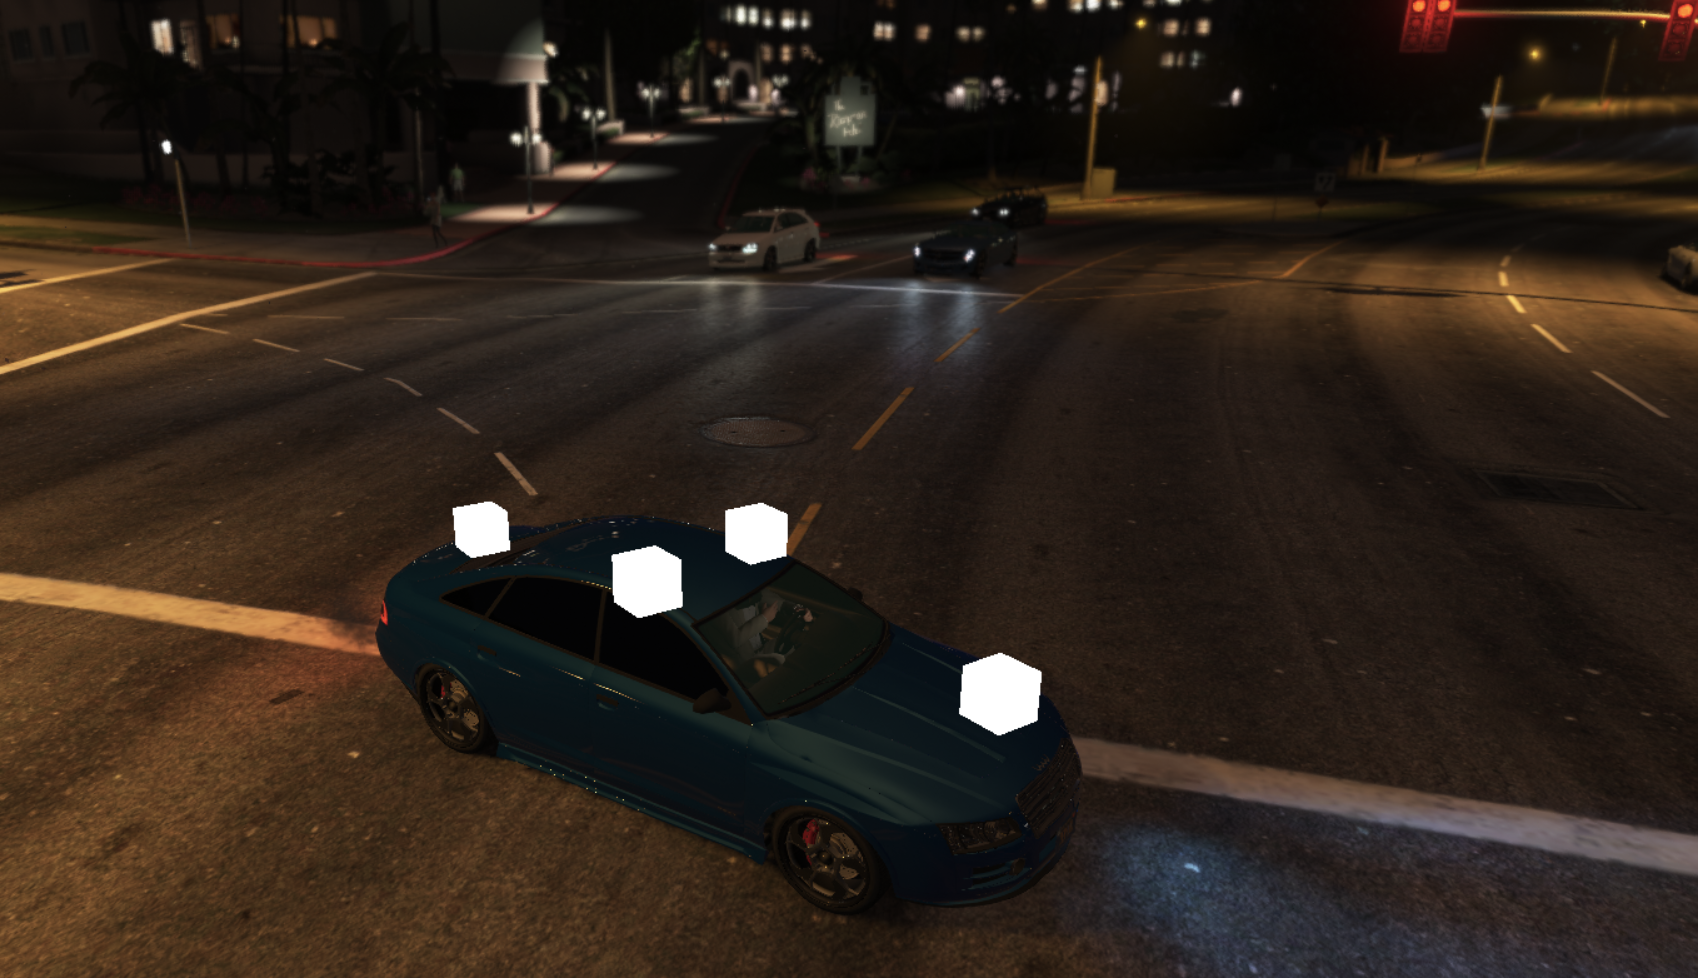
\includegraphics[scale=0.4]{obrazky/dataset-2-cameras}

\caption{\label{fig:Camera-positions-for}Camera positions for second dataset}

\end{figure}


\chapter{3D map estimation}

Restoring 3D map from single image is a complex task. We can think
of depth estimation as preceding problem to the 3D map estimation,
because in depth estimation, we estimate distance of nearest object
pixel-wise, and in 3D map estimation, we have multiple depth levels
per pixel and estimate occupancy per each depth level. The neural
network output is cuboid with size of XxYxZ neurons, hence it is useful
to represent 3D map of a cuboid as a voxel map with X width levels,
Y height levels and Z depth levels. Then we can estimate occupancy
per voxel, in other words, per each neuron output. Thus we can represent
both depth and 3D map estimation as similar instances, depth estimation
being single class occupancy classification per pixel, and 3D map
estimation being multi-class occupancy classification per pixel.

\section{Residual networks}

In machine learning, deep convolutional neural networks have been
used more and more mostly due to significant breakthroughs in image
classification tasks. Advantage of deep neural networks is they are
capable to naturally utilize low-level, mid-level, and high-level
features, without need for manual feature-engineering and lets us
train whole architectures end-to-end. Recent results \cite{going-deeper-with-convolutions,very-deep-image-recognition}
in visual recognition tasks, mostly on ImageNet dataset \cite{imagenet},
reveal depth of network plays crucial role in model accuracy. When
deeper networks were created simply by stacking more and more layers
in the model, these models become hard to train. One of these problems
is the notorious vanishing gradient, which is being addressed by many
approaches, like normalized initialization \cite{efficient-backprop,difficulty-deep-forward}
and normalization layers \cite{batch-normalization}. Other problem
is the degradation problems, where training accuracy starts to worsen,
after stacking more layers \cite{highway-networks}. Residual networks
aim to address this problem of degradation.

If shallower model is able to learn with higher accuracy than deeper
model, we want the deeper model to be able to learn at least same
as shallower one, or better. If we stack new layer into model, we
want them to be able to learn identity mapping. Then the model with
new layers will behave same as shallower model during prediction.
Experiments show that current solvers using gradient descent are not
able to find such solution which would let newer layer to learn identity
mapping in feasible time. The residual learning aims to tackle this
problem by explicitly learning the residual mapping instead of original
mapping. If we want our newly stacked layers to represent mapping
$\mathcal{H}\left(\boldsymbol{x}\right)$, instead we let them learn
another mapping $\mathcal{F}\left(\boldsymbol{x}\right)=\mathcal{H}\left(\boldsymbol{x}\right)-\boldsymbol{x}$.
The original mapping we aim to, $\mathcal{H}\left(\boldsymbol{x}\right)$
is then reconstructed as $\mathcal{H}\left(\boldsymbol{x}\right)=\mathcal{F}\left(\boldsymbol{x}\right)+\boldsymbol{x}$.
He et al. \cite{resnet} shows it is easier to learn the residual
mapping than to learn the original mapping. It also more easily preserves
the identity mapping, if $\mathcal{F}\left(\boldsymbol{x}\right)=\boldsymbol{0}$,
because it is easier to fit these layers to zero than to explicitly
learn identity mapping. 

The formulation of $\mathcal{F}\left(\boldsymbol{x}\right)+\boldsymbol{x}$
can be realized by feed-forward neural network with shortcut connections
\cite{bishop-neural-networks}, also known as skip connections. The
advantage of this approach is it can be easily implemented in current
neural network frameworks out of the box, and it whole network can
still be learned by SGD end-to-end without any further modifications.
Intuitively, the identity mapping, shortcut connection can be seen
as an information highway, where information flows unchanged both
forwards and backwards without any changes. He et al. \cite{resnet}
show the residual learning lets us train very deep models and present
several architectures based on residual learning: ResNet-18, ResNet-34,
Resnet-50, ResNet-101, and ResNet-152. basically ResNet architecture
consists of 4 residual blocks, repeated many times. The difference
between individual architectures is only in number of repetitions
these residual blocks.

\section{Depth estimation}

Depth estimation is one of the most fundamental tasks in computer
vision. Most existing methods \cite{depth-and-surface-estimation,predicting-depth}
formulate depth estimation as a regression task due to the continuous
nature of depth values. Those models for depth estimation are usually
trained to minimize L2 norm between ground truth and predicted depths.
However it shows that regressing to exact depth is difficult task.
In many applications, depth can be known only approximately. With
aforementioned approach, I approximate the regression formulation
of depth estimation with classification problem. Thus instead of training
to predict exact depth, we predict only depth range, still small enough
to be useful for our application. Advantage of classification formulation
of the problem is that after applying soft-max on output of neural
network, depths are naturally predicted as confidence in form of probability
that particular depth level is occupied \cite{depth-estimation-as-classification}.
Most notable methods \cite{depth-estimation-as-classification,depth-estimation-hierarchical-fusion-soft-weighting}
use deep convolutional networks based on famous object classification
architectures. 

Li et al. \cite{depth-estimation-hierarchical-fusion-soft-weighting}
use architecture based on deep residual network \cite{resnet}, specifically
Resnet-152. The architecture is modified, it does not use the fully
connected layer in the end of the network, which drastically decreases
the number of trainable parameters, and instead it appends one convolutional
and one deconvolutional layer. Also, Li et al. utilize the hierarchical
fusion, where output of each block of ResNet is concatenated to other
outputs, with dropout layer afterwards, then the network utilizes
both low-level and high-level features of the input image during the
final layers of depth estimation. The output of final layer is 120x160x200,
meaning it outputs 120x160 pixels image with 200 depth levels. 

Other notable approach of Li et al. is soft weighted sum inference. 

\chapter{Experiments}

\subsection{\label{subsec:Reverse-engineering}Reverse engineering the true Far
Clip}

For reverse engineering the far clip, I gathered 33293 screenshots
with parameters for projection matrix reconstruction and projection
matrices. Because during whole data gathering none of the parameters
used to reconstruct projection matrix, was changed, the projection
matrix should be same for all records. As mentioned in \ref{subsec:Camera-to-NDC}
parameters for reconstructing the Projection matrix are near clip,
far clip, screen width, screen height and field of view.

The screenshot contain both RGB images and depth buffer from GPU.

\begin{figure}
\begin{centering}
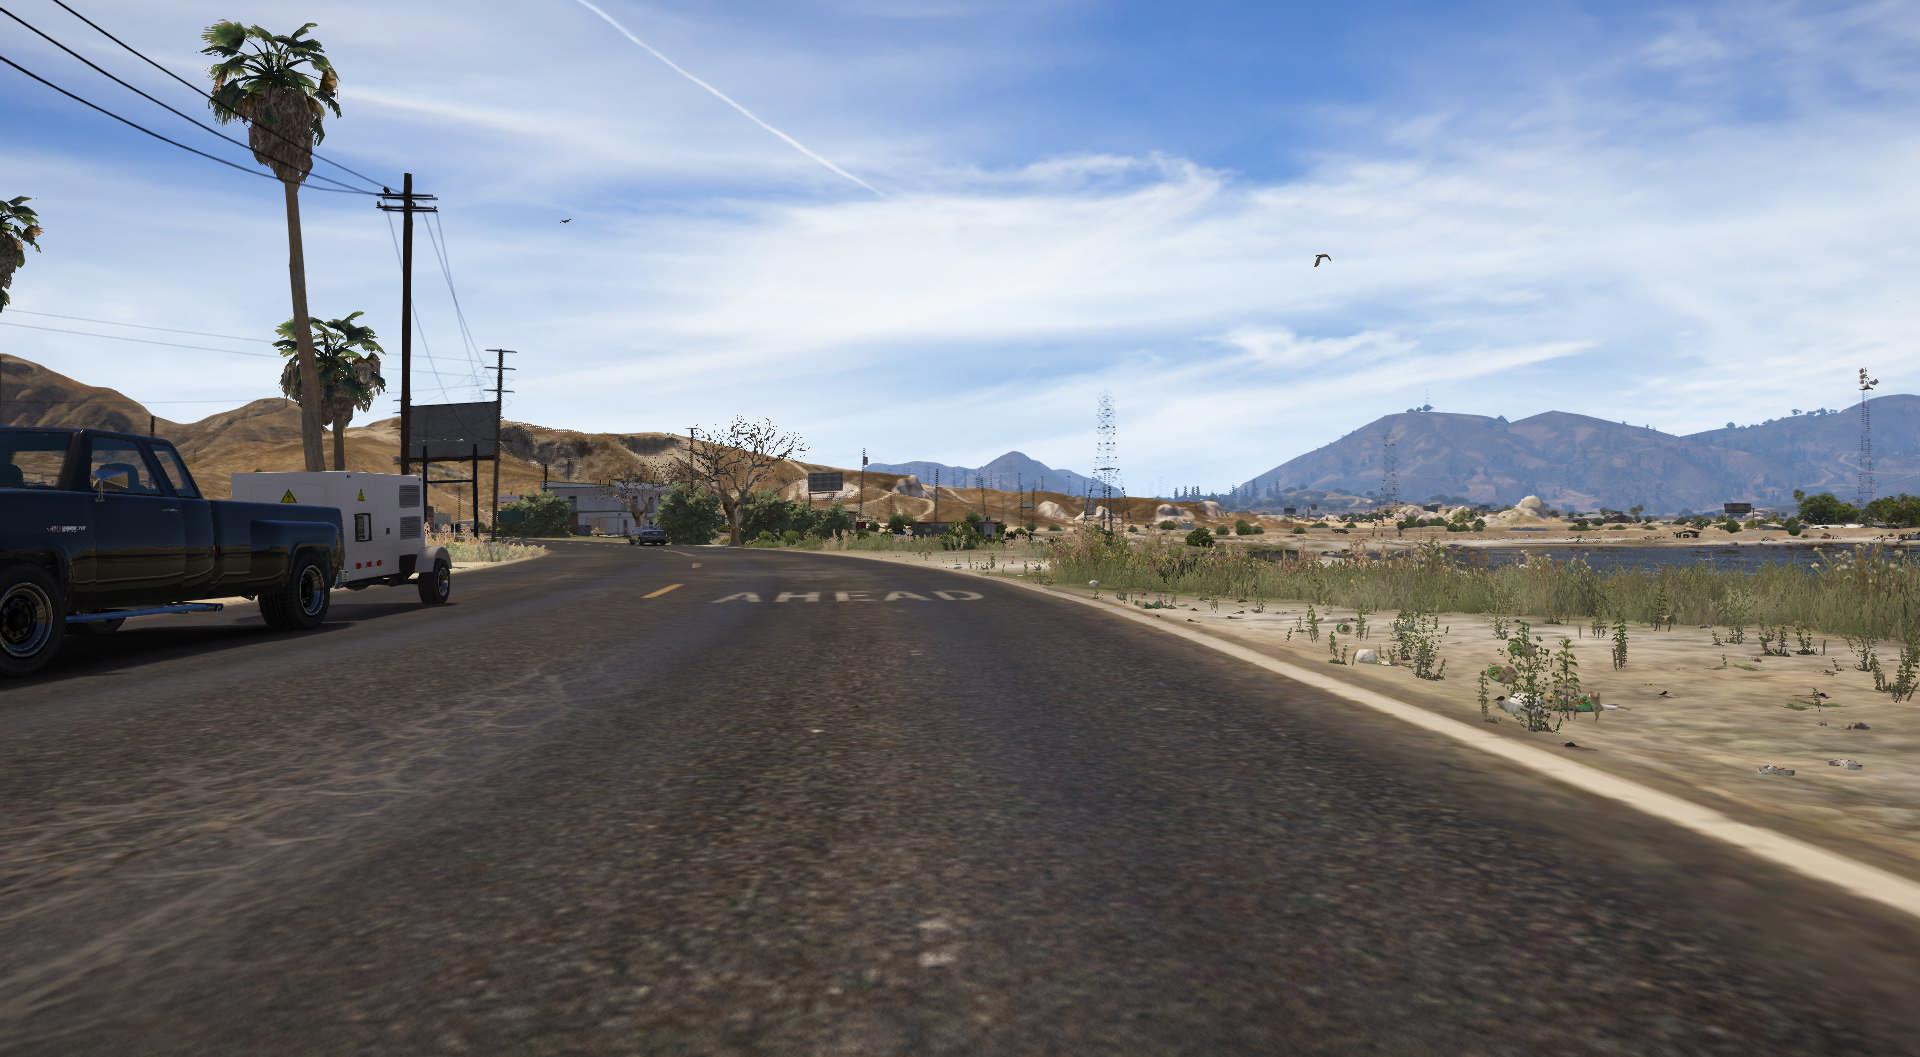
\includegraphics[scale=0.2]{obrazky/2018-03-30--06-00-56--114}
\par\end{centering}
\caption{\label{fig:Example-of-RGB}Example of RGB image}
\end{figure}
\begin{figure}
\begin{centering}
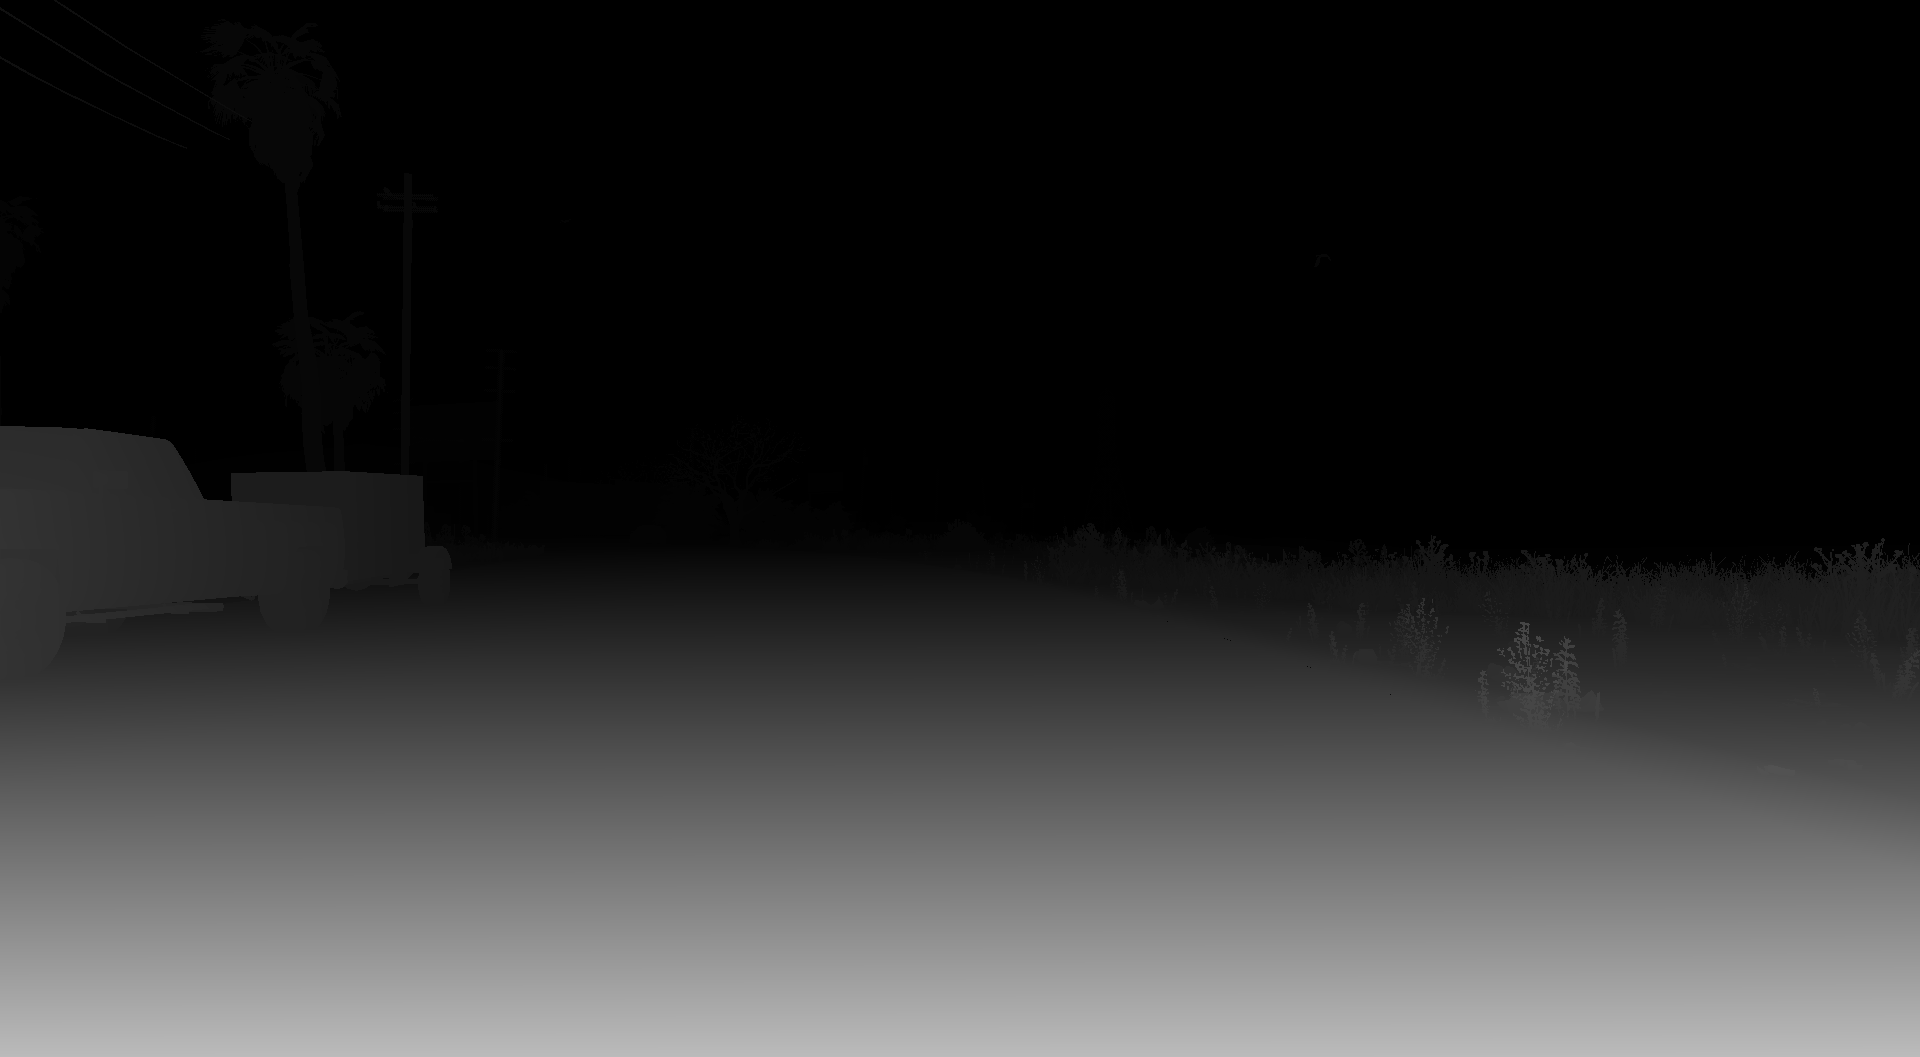
\includegraphics[scale=0.2]{obrazky/2018-03-30--06-00-56--114-depth-8bit-rescaled}
\par\end{centering}
\caption{\label{fig:Example-of-depth}Example of depth buffer}

\end{figure}

The projection matrix transforms frustum into cuboid. Open frameworks
have publicly available projection matrices, but RAGE does not have
publicly available any information about projection matrix, so in
order to obtain true far clip, I needed to reverse-engineer the mathematical
description of the projection matrix. For approximate estimation of
projection matrix parameters, I used DirectX projection matrix\cite{real-time-rendering}
as a starting point for analysis, because GTA V requires DirectX,
so I assumed it is underlying framework of RAGE.

The DirectX projection matrix is 
\[
P^{DirectX}=\begin{bmatrix}\frac{2n}{r-l} & 0 & -\frac{r+l}{r-l} & 0\\
0 & \frac{2n}{t-b} & -\frac{t+b}{t-b} & 0\\
0 & 0 & \frac{f}{f-n} & -\frac{fn}{f-n}\\
0 & 0 & 1 & 0
\end{bmatrix}
\]

where $n$ is near clip, $f$ is far clip, $l$ and $r$ determine
distance between left and right planes of the frustum and $t$ and
$b$ determine distance between top and bottom planes.

The view frustum is symmetric, so $r=-l$ and $t=-b$ \cite{real-time-rendering}.
In that case, the projection matrix is simplified to form
\[
P^{formal}=\begin{bmatrix}\frac{2n}{r+r} & 0 & -\frac{r-r}{r+r} & 0\\
0 & \frac{2n}{t+t} & -\frac{t-t}{t+t} & 0\\
0 & 0 & \frac{f}{f-n} & -\frac{fn}{f-n}\\
0 & 0 & 1 & 0
\end{bmatrix}=\begin{bmatrix}\frac{n}{r} & 0 & 0 & 0\\
0 & \frac{n}{t} & 0 & 0\\
0 & 0 & \frac{f}{f-n} & -\frac{fn}{f-n}\\
0 & 0 & 1 & 0
\end{bmatrix}
\]
The DirectX maps near clip to 0 and far clip to 1, but from data,
where obviously\ref{fig:Example-of-depth} nearer pixels had higher
value in depth buffer than pixel more far from camera, I concluded
that near and far clip are being mapped to 1 and 0, respectively.
The far clip being mapped to 0 can also be deduced by pixels for sky
having 0 value.

Due to this fact, we switch the near and clip in the matrix formal
description

\[
P^{formal}=\begin{bmatrix}\frac{f}{r} & 0 & 0 & 0\\
0 & \frac{f}{t} & 0 & 0\\
0 & 0 & \frac{n}{n-f} & -\frac{fn}{n-f}\\
0 & 0 & 1 & 0
\end{bmatrix}
\]

The example in \ref{fig:Example-of-depth} does not have actual depth
buffer values, but instead, it is rescaled visualization. Since the
depth buffer pixels are in range $\left[0,1\right]$ and PNG images
take unsigned 8bit integer, this image is mapped linearly from $\left[0,1\right]$
to $\left[0,255\right]$. Since even the nearest pixels were distant
from near clip and real range of pixels in this image was $\left[0,19\right]$,
I rescaled it 10 times to range $\left[0,190\right]$, so the depth
is visible.

At first, I assumed the camera near clip and far clip obtained by
native calls \ref{native-call-near-clip} and the projection matrix
is same as in DirectX. 

The near clip and far clip calculation can be demonstrated on image
\ref{fig:Example-of-RGB}. 

By calling CAM::GET\_CAM\_NEAR\_CLIP$=n_{c}$ and CAM::GET\_CAM\_FAR\_CLIP$=f_{c}$
I obtained values $n_{c}=1.5$ and $f_{c}=800$. I also obtain projection
matrix calculated by method described in \ref{subsec:Rendering-pipeline-data},
which is 
\[
P^{real}=\begin{bmatrix}1.210067 & 0 & 0 & -0.000004\\
0 & 2.144507 & 0 & 0.000002\\
0 & 0 & 0.00015 & 1.500225\\
0 & 0 & -1 & 0
\end{bmatrix}
\]

In the formalization of the matrix, $P_{formal}$, there are 4 variables.
$r$ and $t$ appear only in one element of matrix, so they can be
verified only after reverse engineering the far clip. From the $P_{2,2}^{formal}$
and $P_{2,3}^{formal}$, I can calculate the near and far clip by
\begin{align*}
P_{2,2}^{formal} & =\frac{n}{n-f}\\
nP_{2,2}^{formal}-fP_{2,2}^{formal} & =n\\
\frac{n\left(P_{2,2}^{formal}-1\right)}{P_{2,2}^{formal}} & =f
\end{align*}

\begin{align*}
P_{2,3}^{formal} & =-\frac{fn}{n-f}\\
P_{2,3}^{formal}\left(n-f\right) & =-fn\\
nP_{2,3}^{formal} & =f\left(P_{2,3}^{formal}-n\right)\\
\frac{nP_{2,3}^{formal}}{\left(P_{2,3}^{formal}-n\right)} & =f
\end{align*}
\begin{align*}
\frac{nP_{2,3}^{formal}}{\left(P_{2,3}^{formal}-n\right)} & =\frac{n\left(P_{2,2}^{formal}-1\right)}{P_{2,2}^{formal}}\\
P_{2,3}^{formal}P_{2,2}^{formal} & =\left(P_{2,2}^{formal}-1\right)\left(P_{2,3}^{formal}-n\right)\\
\frac{P_{2,3}^{formal}P_{2,2}^{formal}}{P_{2,2}^{formal}-1} & =P_{2,3}^{formal}-n\\
P_{2,3}^{formal}-\frac{P_{2,3}^{formal}P_{2,2}^{formal}}{P_{2,2}^{formal}-1} & =n\\
-\frac{P_{2,3}^{formal}}{P_{2,2}^{formal}-1} & =n
\end{align*}

\begin{align*}
\frac{\left(-\frac{P_{2,3}^{formal}}{P_{2,2}^{formal}-1}\right)\left(P_{2,2}^{formal}-1\right)}{P_{2,2}^{formal}} & =f\\
-\frac{P_{2,3}^{formal}}{P_{2,2}^{formal}} & =f
\end{align*}

From these calculations, we can calculate near and far clip as 
\begin{align*}
n & =-\frac{P_{2,3}^{formal}}{P_{2,2}^{formal}-1}=-\frac{1.500225}{0.00015-1}=1.500225\\
f & =-\frac{P_{2,3}^{formal}}{P_{2,2}^{formal}}=-\frac{1.500225}{0.00015}=-10001.5
\end{align*}

From these calculations we can see the third column of the projection
matrix has incorrect sign, because the $P_{3,2}^{formal}$ should
be 1 and instead it is -1, and the far clip is negative, which should
not be. When changing signs of third column of projection matrix,
we obtain following formal definition of projection matrix. That sign
switching means the view frustum is in opposite direction of Z axis.
\[
P^{formal}=\begin{bmatrix}\frac{f}{r} & 0 & 0 & 0\\
0 & \frac{f}{t} & 0 & 0\\
0 & 0 & -\frac{n}{n-f} & -\frac{fn}{n-f}\\
0 & 0 & -1 & 0
\end{bmatrix}
\]

After fixing the sign issue, the relationship between $P^{formal}$
and clips is

\begin{align*}
\frac{P_{2,3}^{formal}}{P_{2,2}^{formal}+1} & =n=\frac{1.500225}{0.00015+1}=1.499999\\
\frac{P_{2,3}^{formal}}{P_{2,2}^{formal}} & =f=\frac{1.500225}{0.00015}=10001.5
\end{align*}

As we can see, the $n=1.499999\approx n_{c}=1.5$ so for near clip,
we can say we successfully reverse-engineered the relation between
the projection matrix and the near clip. The far clip, on the other
hand, differs $f=10001.5\neq f_{c}=800$. The difference is very high,
which lead us to assumption that there is some new far clip, which
is not same as obtained through API, $f_{c}$. 

The other check we can perform is projecting points laying on near
clip and far clip into NDC space. 

We prepare two points. Because of many zero elements in $P^{formal}$,
we can see $x$-axis and $y$-axis don't affect the $z$-axis of projected
point. Thus I prepared two points:
\[
\begin{bmatrix}1 & 1\\
1 & 1\\
-1.5 & -800\\
1 & 1
\end{bmatrix}
\]
, which are laying on the near clip and far clip, respectively. We
would assume that they would be mapped to 1 and 0, respectively. The
negative sign is here because in RAGE, the camera view frustum is
in negative part of Z axis.

\[
\begin{bmatrix}1.210067 & 0 & 0 & -0.000004\\
0 & 2.144507 & 0 & 0.000002\\
0 & 0 & 0.00015 & 1.500225\\
0 & 0 & -1 & 0
\end{bmatrix}\begin{bmatrix}1 & 1\\
1 & 1\\
-0.15 & -800\\
1 & 1
\end{bmatrix}=\begin{bmatrix}1.210063 & 1.210063\\
2.144509 & 2.144509\\
1.5 & 1.380225\\
1.5 & 800
\end{bmatrix}
\]
by normalization we obtain 
\[
\begin{bmatrix}\frac{1.210063}{1.5} & \frac{1.210063}{800}\\
\frac{2.144509}{1.5} & \frac{2.144509}{800}\\
\frac{1.50045}{1.5} & \frac{1.620225}{800}\\
\frac{1.5}{1.5} & \frac{800}{800}
\end{bmatrix}=\begin{bmatrix}0.80670867 & 0.00151258\\
1.42967267 & 0.00268064\\
1 & 0.00172528\\
1 & 1
\end{bmatrix}
\]
from which we can see the near clip $n_{c}$ is being projected correctly,
but far clip $f_{c}$ is not being projected into 0 and that true
far clip $f$ is behind this far flip $f_{c}$.

These calculations give us some insight into projection matrix and
its role in far clip estimation, but for more robust estimate, I analysed
all 33293 matrices. 

In GTA, matrices are not gathered correctly every time and in some
cases, resulting matrices are unusable. Because I knew the near clip
precisely, I discarded all matrices, with calculated near clip $\left|n-n_{c}\right|>10^{-4}$.

\chapter{Future work}

In GTA V reverse-engineering, many stencil values semantics remain
to be discovered. 

\bibliographystyle{plainnat}
\phantomsection\addcontentsline{toc}{chapter}{\bibname}\bibliography{bibliography}


\appendix

\chapter{Contents of the enclosed CD}

\inputencoding{latin9}\begin{lstlisting}
appendix content
\end{lstlisting}
\inputencoding{utf8}
\cleardoublepage{}
\end{document}
